\documentclass[12pt,lettersize]{book}
\usepackage{amsmath, amsthm, amscd}
\usepackage{tikz}
\usetikzlibrary{matrix,chains,positioning,decorations.pathreplacing,arrows}
\usepackage{graphicx}
\usepackage{algorithmicx} 
\usepackage{algpseudocode}
\usepackage{algorithm}
%\usepackage{fancyhdr}
%\usepackage[colorlinks=true,linkcolor=cyan]{hyperref}

% Strike line
\usepackage{ulem}
\usepackage{caption}

% Subfigure
\usepackage{subcaption}
\usepackage{booktabs}

% Syntax tree
\usepackage{qtree}
\usepackage[margin=2cm]{geometry}

% Paragraph
\usepackage{parskip}

% Page number
\usepackage{lastpage}

% Line space
\usepackage{setspace}

% Font
\renewcommand*\rmdefault{ppl}
%\usepackage{times}

% Macros
% Partial derivatives
\newcommand{\del}{\partial}
% Norm
\newcommand\norm[1]{\left\lVert#1\right\rVert}
% Matrix/vector bold fonts
\newcommand{\+}[1]{\ensuremath{\mathbf{#1}}}
% Transpose
\newcommand{\tran}{^{\mathstrut\scriptscriptstyle\top}} 
% Algorithm input/output
\renewcommand{\algorithmicrequire}{\textbf{input:}}
\renewcommand{\algorithmicensure}{\textbf{output:}}
\setlength{\parskip}{0.5em}
\onehalfspace

\newcommand{\HRule}{\rule{\linewidth}{0.5mm}}
\title{Image-Based Question Answering with Visual Semantic Embeddings}
\date{\today}
\author{Mengye Ren}
\begin{document}
\begin{titlepage}
\hfill\\
\hfill\\
\hfill\\
\hfill\\
\hfill\\
\hfill\\
\hfill\\
\begin{center}
\Large Image-Based Question Answering with Visual Semantic Embeddings\\
\hfill\\
\normalsize by\\
\hfill\\
Mengye Ren\\
\hfill\\
\hfill\\
Supervisor: Richard S. Zemel\\
\today
\end{center}
\vspace*{\fill}
\end{titlepage}
\setcounter{page}{1}
\pagenumbering{roman}
\chapter*{Abstract}
Computers understanding complex objects in an image and interacting with human through natural language are two open areas of research in computer vision and computational linguistics. A three-year-old child can describe what he/she sees and answer questions regarding to the visual elements, but computers have an extraordinarily hard time handling these simple tasks. Learning and applying visual and semantic knowledge in a computer program will mean a big step in the field of artificial intelligence.

This work, image-based question answering with visual semantic embeddings, aims to let computers jointly learn both vision and natural language through a question-answering (QA) task. In recent years, we have evidenced major breakthroughs in deep learning, machine learning models of deep neural networks, on applications such as object recognition and natural language processing. Inpired by previous approaches using convolutional and recurrent neural networks \cite{simonyan14, krizhevsky12, sutskever14, kiros14b}, we combined these learning architectures to create a common embedding space -- a visual semantic embedding to represent both images and sentences. We designed models that learn to perform question-answering task within this common embedding space.

Image-based question answering is still a fairly new field. We show that our proposed models achieved more than 1.5 times better accuracy compared to the previous effort \cite{malinowski14b} on the same dataset \cite{malinowski14b}. To further evaluate our models and to contribute more data to the research community, we are releasing another dataset that is 20 times larger by converting an image description dataset \cite{mscoco} into question-answer forms. We hope that our work can encourage more follow-up research to achieve better results than ours.

The five chapters will be organized as follows: Chapter 1 will give a brief introduction on the motivation of developing image-based question answering technology. Chapter 2 will cover both the technical backgrounds of our proposed methods, i.e. neural networks and word embeddings, and previous attempts on this very topic. Chapter 3 will explain our neural network medels and our dataset generation algorithms in detail and present the results. Chapter 4 will discuss the significance of our results and Chapter 5 will present some future directions of this research. 
\chapter*{Acknowledgements}
This thesis would not have been possible without the guidance and support of many people. 

First, I would like to thank my advisor Dr. Richard Zemel. Dr. Zemel brought me into the research gate of machine learning when I still did not know anything about it. He suggested such an interesting research project to me that I had never believed I could work on it. Throughout the final year of my undergraduate studies, he always encouraged me on any little progress I made. He gave me many new directions and resources that lead to results of this research.

I owe many thanks to my mentor Ryan Kiros, who is a PhD student in the machine learning group. Ryan has spent a lot of time helping me on this thesis, and has inspired me with a lot of his brilliant ideas on the model design. His energetic attitude also influenced me. Without Ryan's guidance, I certainly would not have achieved as many results. 

I also want to thank Dr. Ruslan Salakhutdinov for a helpful discussion on the bidirectional models, and Nitish Srivastava for his support on the Toronto Conv Net. Nitish's excellent Conv Net software and trained models really made my research easy to get started.  Of course, my research would not have been feasible without the computing resources. Dr. Zemel did not have any hesitation assigning me with all the computing resources I needed, and I am thankful to Dr. Relu Patrascu for setting up my account and access to the computing clusters. 

I would like to thank everyone in the machine learning group at the University of Toronto. I benefited a lot from attending the weekly cookie talks and paper discussions. They really broadened my knowledge on the cutting-edge research in the machine learning community.

I would like to say thank you to all of my friends in Engineering Science. I enjoyed the four years of fruitful undergraduate studies with you and I will be very proud of being an Engineering Science alumnus.

Finally, I would like to thank my parents Yue Li and Lizhi Ren. I thank their love and support to let me explore in the area of my interest and passion. 
\tableofcontents
\listoftables
\listoffigures
\setcounter{page}{1}
\pagenumbering{arabic}
\chapter{Introduction}
Vision and language are two major inputs of human perception. Everyday, we see images through eyes and listen to speech through ears, and often the two are associated and complementary to each other. Speakers use visual elements such as projector slides to make their lectures easier to understand, and photographers use captions and descriptions to convey deeper thoughts of their photos. 

However, compared to humans, computers are extremely poor at vision and language. A human can recognize objects in each part of the image and describe them using his/her own words, but it is still a very difficult task for computers. In recent years, computational models, pariticularly large-scale deep convolutional and recurrent neural networks, have achieved eminent success in the field of object recognition and natural language processing \cite{simonyan14, krizhevsky12, sutskever14, kiros14b}. The achievement from previous research has formed the building blocks of learning higher level representations of vision and language.

In this work, we hope to design machine learning models that can jointly learn vision and language through a question-answering (QA) task. The computer is given a set of images and questions regarding the images, and is expected to output correct answers through a supervised learning scheme. Machines need to combine knowledge from both image and words in order to achieve good performance.

Building an image-based question answering system has profound implication in the field of artificial intelligence (AI). Natural language human-computer interation eliminates the need for prerequisite knowledge of operating electronic devices, which will make technologies more accessible. Exchanging image understanding through natural language can also bring benefits to users with visual disabilities. Image-based question answering technology will trigger countless AI applications and can be directly deployed in robots and wearables to assist humans on daily basis.

Tackling the problem is not an easy task, due to multiple layers of complexity. Not only does the model need to parse the scenes and objects in the image, it also needs to understand the question and generate the relevant answer. Compared to image description generation, image QA requires answers to be targeted to the questions with higher precision. 
Image QA is still a fairly new field. The current available datasets were just released last December \cite{malinowski14a}. The authors also presented their approach to this problem, which can be improved by a large margin. In short, there is a lack of large and high-quality datasets as well as competitive models on this problem.

Our goal is to design a machine learning model that learns a representation combining both images and sentences. Unlike the existing approach, we formulate the problem using embedding spaces. First, we need to convert the images and questions into vector forms so that they can be sent as inputs to a neural network. We propose to use the state-of-the-art convolutional neural networks to obtain the visual features, and use recurrent neural networks to obtain sentence-level embedding. We will cover the basics of neural networks and embedding models in Chapter \ref{background}. Now, we can reduce the problem into a multi-class classification problem by assuming only single-word answers. We aim to learn a function that outputs either the answer class or the nearest neighbour of the correct answer in the semantic embedding space. Lastly, as the currently available dataset may be insufficient for our approach, we propose an automatic question generation algorithm to synthesize QA pairs from a large image description dataset.

In conclusion, solving the problem of image-based question answering will be a meaningful step in the field of machine learning and AI. We hope this work will invite more research in the future linking computer vision and natural language knowledge in a broader sense.

\section{Overview of the thesis}

Chapter 2 will introduce the background of our proposed methodology, including the very basics of neural networks and word embeddings as well as more recent research on jointly learning image and text with neural network based embedding models. Chapter 3 will describe our proposed approaches and results. We will explain the models in detail with their performance. We will present an algorithm that helps us collecting a large scale image QA dataset. Chapter 4 will discuss the experimental results in depth, and lastly Chapter 5 will propose future work on our line of research.
\chapter{Background}
\label{background}
Deep architecture and recurrent topology have been significantly developed over the last decade that allow neural networks to automatically extract abstract and useful features. They are as of today the best tools to solve problems such as image detection \cite{krizhevsky12, girshick14}, speech recognition \cite{dahl12, deng13}, and language modelling \cite{mnih07, mikolov10}, outperforming many known machine learning models with hand-crafted feature-extractors. Since our model formulation relies mainly on deep neural networks, this chapter will begin with the basics of neural networks. 

\section{Neural networks}
Artificial neural networks are computational models that consist of interconnected adaptive units \cite{hassoun03}. A set of input is feeded to each unit, also called artificial neuron, with certain weights assigned. 

\begin{figure}
\centering
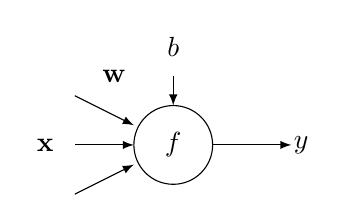
\begin{tikzpicture}[scale=2.5]
\draw (0, 0) circle (0.2cm);
\draw [-latex] (-0.5, 0.25) -- (-0.2, 0.1);
\draw [-latex] (-0.5, 0) -- (-0.2, 0);
\draw [-latex] (-0.5, -0.25) -- (-0.2, -0.1);
\draw [-latex] (0, 0.35) -- (0, 0.2);
\draw [-latex] (0.2, 0) -- (0.6, 0);
\path (0,0.5) node[draw=none] (b) {$b$};
\path (-0.3,0.35) node[draw=none] (w) {$\ensuremath{\mathbf{w}}$};
\path (-0.65,0) node[draw=none] (x) {$\ensuremath{\mathbf{x}}$};
\path (0.65,0) node[draw=none] (y) {$y$};
\path (0,0) node[draw=none] (f) {$f$};
\end{tikzpicture}
\caption{An artificial neuron}
\label{fig:neuron}
\end{figure}

Each neuron takes the weighted sum of the input, with an optional bias term, and applies an activation function. It is an intuition borrowed from neuroscience: a neuron is fired after the electric current passes some threshold.

\begin{equation}
z = \+w\tran\+x + b
\end{equation}

$\+x$ is an input vector with dimension $D$, and $\+w$ is a weight vector also of dimension $D$, and $b$ is a scalar bias term.

\begin{equation}
y = f(z)=f(\+w\tran\+x + b)
\end{equation}

A common activation function are the sigmoid function: $f(z) = \dfrac{1}{1+e^{-z}}$, and the hyperbolic tangent function: $f(z) = \tanh(z)$. As shown in \ref{fig:sigmoid}, the sigmoid function is in its ``on'' state with output to be approximately one on the far right, and in its ``off'' state with output to be approximately zero on the far left. There is a linear region around the origin where the output climbs from zero to one. 

\begin{figure}
\centering

\begin{tikzpicture}[domain=-3:3, xscale=1.5, yscale=3.5]
    \draw[->] (-3,0) -- (3,0) node[right] {$z$}; 
    \draw[->] (0,0) -- (0,1.1) node[above] {$f(z)$};
	\draw plot (\x,{1/(1+exp(-\x))}) node[right] {}; 
	% ticks
	\foreach \x in {-2,...,2}
 		\draw (\x,1pt) -- (\x,-3pt)
		node[anchor=north] {\x};
	\foreach \y in {1}
 		\draw (1pt,\y) -- (-3pt,\y) 
 		node[anchor=east] {\y}; 
\end{tikzpicture}
\caption{The sigmoid function}
\label{fig:sigmoid}
\end{figure}

\subsection{Feedforward neural networks}
A feedforward neural network is composed of layers of parallel neurons that process input and transmits data to the next layer. In terms of network topology, a typical feedforward neural network can be decomposed into three types of layers: one input layer, possibly multiple hidden layers, and one output layer. The input layer contains simply the original data samples. The hidden layer and the output layer neurons contain activation functions. We present equations for a single hidden layer network below.

\begin{equation}
\begin{array}{r c l}
\+h &=& f^{(1)}(\+W^{(1)}\+x + \+b^{(1)})\\
\+y &=& f^{(2)}(\+W^{(2)}\+h + \+b^{(2)})
\end{array}
\end{equation}

$f^{(1)}$ and $f^{(2)}$ are activation functions for the hidden layer and the output layer, which can be different functions. $\+W^{(1)}$ is the weight matrix from the input layer to the hidden layer with dimension $H \times D$, where $D$ is the input dimension and $H$ is the hidden dimension. $\+x$ is the input vector of the neural network and $\+y$ is the output vector. With a nonlinear activation function such as the sigmoid function, a single hidden layer neural network is proved to have  capability of universal function approximation \cite{du2014}. 

\begin{figure}
\centering
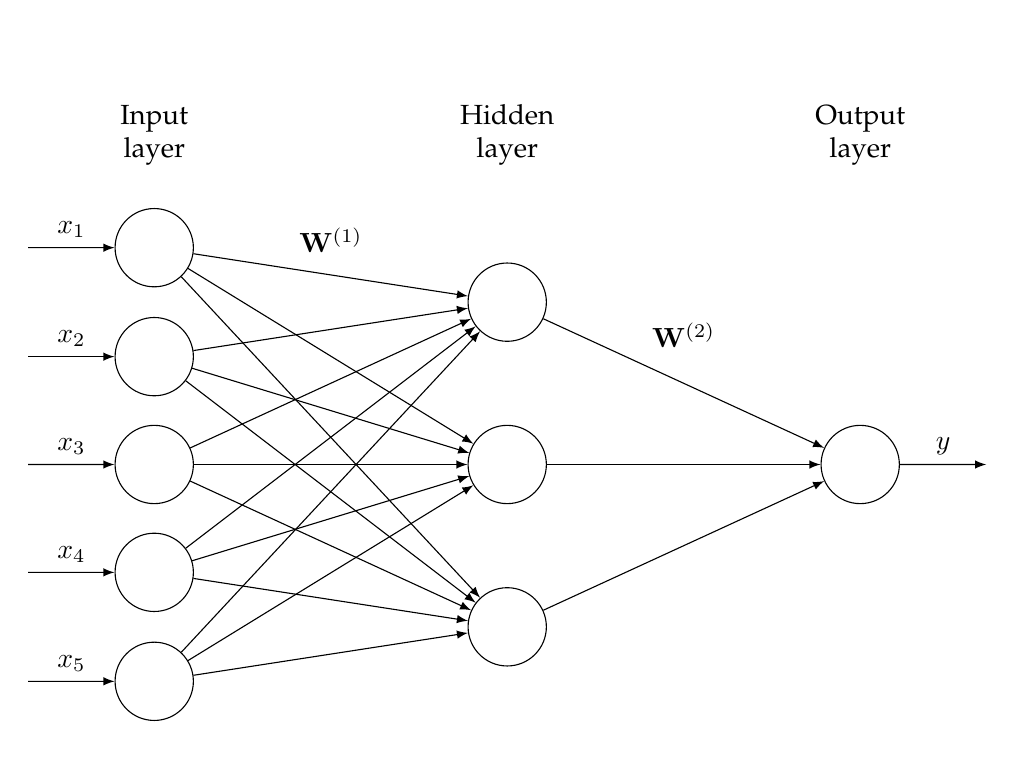
\begin{tikzpicture}[
plain/.style={
  draw=none,
  fill=none,
  },
net/.style={
  matrix of nodes,
  nodes={
    draw,
    circle,
    inner sep=10pt
    },
  nodes in empty cells,
  column sep=2cm,
  row sep=-9pt
  },
>=latex,scale=0.8
]
\matrix[net] (mat)
{
|[plain]| \parbox{1.3cm}{\centering Input\\layer} & |[plain]| \parbox{1.3cm}{\centering Hidden\\layer} & |[plain]| \parbox{1.3cm}{\centering Output\\layer} \\
& |[plain]| \\
|[plain]| & \\
& |[plain]| \\
|[plain]| & |[plain]| \\
& & \\
|[plain]| & |[plain]| \\
& |[plain]| \\
|[plain]| & \\
& |[plain]| \\
};
\foreach \ai [count=\mi ]in {2,4,...,10}
  \draw[<-] (mat-\ai-1) -- node[above] {$x_\mi$} +(-2cm,0);
\foreach \ai in {2,4,...,10}
{\foreach \aii in {3,6,9}
  \draw[->] (mat-\ai-1) -- (mat-\aii-2);
}
\foreach \ai in {3,6,9}
  \draw[->] (mat-\ai-2) -- (mat-6-3);
\draw[->] (mat-6-3) -- node[above] {$y$} +(2cm,0);

\path (-2.8,2.2) node[draw=none] (X1) {$\ensuremath{\mathbf{W}}^{(1)}$};
\path (2.8,0.7) node[draw=none] (X1) {$\ensuremath{\mathbf{W}}^{(2)}$};
\end{tikzpicture}


\caption{A feedforward net with one hidden layer (adapted from \cite{ffnn})}
\label{fig:ffnet}
\end{figure}


\subsection{Error functions}

We first define the error function as some measure of cost from the network output to the desired output. For example, the sum of square error is defined as following:

\begin{equation}
E(\+y) = \sum_i (t_i - y_i)^2
\end{equation}

$\+y$ is the network output, and $\+t$ is the desired output, or the ground truth in the training dataset. $i$ denotes the index of the output element. For classification problems, usually the output is the probability of an example belonging to a class. It is more common to use the cross-entropy error function for this type of problems. For binary classification, the cross-entropy is defined as following:

\begin{equation}
E(\+y) = \sum_i  - t_i \log(y_i) - (1 - t_i) \log(y_i)
\end{equation}

$t$ and $y$ have the same definition as above. $t = 1$ means the example belongs to class $1$ and $0$ means class $0$. If the output of the network is exactly the same with the ground truth, the value of the error function will be zero, and if the output is exactly the opposite, the value of the error function goes to infinity. For multiple class problems, the activation function is usually a softmax function, also called normalized exponential:

\begin{equation}
\+y = \dfrac{e^\+z}{\sum_i e^{z_i}}
\end{equation}

where $z$ is the activation value before output and $i$ denotes the index of the output element. In this way, the class with the maximum probability is preserved and the function is differentiable. The multi-class cross-entropy error function is defined as following:

\begin{equation}
E(\+y) = \sum_i -t_i \log(y_i)
\end{equation}

$\+t$ is a vector with all zeros except one entry with the correct class of the example, and $\+y$ is a vector of the network predicted class probability. This can be seen as an extension to the two-class case.

\subsection{Training neural networks}
%\subsection{Backpropagation}
The training of neural networks is usually achieved through backpropagation. Equivalently speaking, learning can be regarded as a minimization problem of some error function, and backpropagation a first-order gradient descent method. The calculus chain rule is used to derive the error derivative with regard to weights in each layer. For each update, we take a small step of the gradient towards lower value of the error function.

\begin{equation}
\dfrac{\del E}{\del \+w} = \sum_i \dfrac{\del E}{\del y_i} \dfrac{\del y_i}{\del \+w}
\end{equation}

\begin{equation}
\+w_{t+1} = \+w_{t} - \gamma \left(\dfrac{\del E}{\del \+w}\right)_t
\end{equation}

$\gamma$ is also called the learning rate or the step size. If we have want to further backpropagate to previous layers of neurons, we need to use the chain rule again to calculate the error derivative with regard to the input of the current layer.

\begin{equation}
\dfrac{\del E}{\del x_j} = \sum_i \dfrac{\del E}{\del y_i} \dfrac{\del y_i}{\del x_j}
\end{equation}

More neural networks training techniques can be found in Appendix~\ref{train_tech}.

\subsection{Convolutional neural networks (CNNs)}
One obvious advantage of neural network is fighting against the curse of dimensionality. For example, a small image patch of 28 pixel $\times$ 28 pixel with binary pixel values will generate $2^{28 \times 28} = 2^{784}$ different possible images. In the classic MNIST handwritten digit dataset \cite{lecun98}, there are only sixty thousand training examples. Neural networks can learn the input-output relation with a continuous function that has the ability of generalize to unseen data. 

However, one hidden layer neural networks still has its limitations. To achieve larger learning capacity, a large number of hidden neurons are required, but this also increases the total number of weights need to be learned. With only small number of examples, a neural network quickly overfits the training set, and perform poorly on the test set. Weight sharing is an important technique to preserve the generalization ability. The idea is to force some weights the same across the entire learning process, which is often done through summing all the error derivatives for those shared weights and update them with the sum. Convolutional neural networks \cite{lecun98}, is exactly built on top of the the idea of weight sharing. LeNet \cite{lecun98}, one of the first CNNs, achieved the highest MNIST handwritten digit classification rate at the time. 

\begin{figure}
\includegraphics[width=\textwidth]{cnn.png}
\caption{A convolutional neural net \cite{cnn}}
\label{fig:cnn}
\end{figure}

\begin{figure}
\includegraphics[width=\textwidth]{filters.png}
\caption{Automatically learned low-level image filters \cite{krizhevsky12}}
\label{fig:cnn_filters}
\end{figure}

The flipped version of the shared weights can be regarded as small square shape image filters (Figure~\ref{fig:cnn_filters}), and the computation to each hidden neurons is equivalent to a 2-D convolution on the original image. Filtered images are then passed to a Rectified Linear Unit (ReLU) ($f(z) = \max\{0, z\}$) to obtain non­linear activation to certain features. Next, to reduce data dimensionality and to make the model robust to translational invariance, a max pooling layer effectively downsamples the intermediate image with the maximum value in each subregion. Lastly, a fully connected softmax layer makes class predictions with each unit representing the probability of input data belonging to certain classes. Such deep architecture has achieved the state of the art image classification and detection results in recent object classification and detection competitions \cite{krizhevsky12, girshick14}. Figure~\ref{fig:cnn} shows a typical CNN architecture. 

\subsection{Recurrent neural networks (RNNs)}

Recurrent neural network is a type of network that sends the output back to the input neurons, creating feedbacks in the network topology. It is designed to learn time series input because time dependency features can be effectively captured by the feedback loop. Recently, recurrent neural networks have been applied on many natural language tasks, such as language modelling, machine translation, etc. This thesis will focus on one popular type of recurrent neural network called long short-term memory (LSTM), and we will use it as our sentence model.

\begin{figure}
\centering
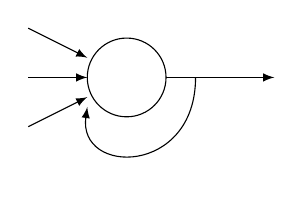
\begin{tikzpicture}[scale=2.5]
\draw (0, 0) circle (0.2cm);
\draw [-latex] (0.35, 0) .. controls (0.35, -0.5) and (-0.25, -0.5) .. (-0.2, -0.15);
\draw [-latex] (-0.5, 0.25) -- (-0.2, 0.1);
\draw [-latex] (-0.5, 0) -- (-0.2, 0);
\draw [-latex] (-0.5, -0.25) -- (-0.2, -0.1);
\draw [-latex] (0.2, 0) -- (0.75, 0);
\end{tikzpicture}
\caption{A recurrent neuron with a feedback loop}
\label{fig:rnn}
\end{figure}

\subsection{Long short-term memory (LSTM)}
Long short-term memory (LSTM) \cite{hochreiter97} is a major variant of recurrent neural networks. The training of regular RNNs is notoriously difficult because of the vanishing and exploding gradients problems. LSTM is designed to address these training issues. One of the main feature of LSTM is the constant error propagation in its memory unit. This is brought by the linear activation of the memory content at every timestep. But this also results in a complex structure as in shown Fig~\ref{fig:lstm}.

LSTM has a central memory unit ($\+c$) with three different types of multiplicative gating that controls the flow of information in the memory. The value of each gating at every time step is determined by a weighted sum of the current input ($\+x_t$), the current memory content ($\+c_t$), and the current output ($\+y_t$). A sigmoid function maps the weighted sum to a gating value between zero and one. The memory of each timestep is then updated by the forget gate ($\+f_t$) multiplying with the memory content from the previous time step, and the input gate ($\+i_t$) multiplying with the current input through a hyperbolic tangent (tanh) activation function. Lastly, the output of the neural network can be obtained by the output gate ($\+o_t$) multiplying with the current memory through another hyperbolic tangent activation. The equations of LSTM are summarized in Equation~\ref{eq:lstm}.

\begin{figure}
\centering
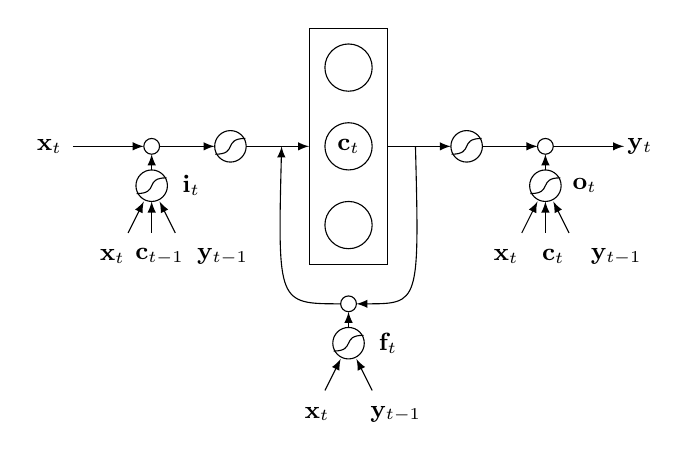
\begin{tikzpicture}[font=\small]

% Central memory unit
\draw (0,0) rectangle (1,3);
\draw (0.5,2.5) circle (0.3cm);
\draw (0.5,1.5) circle (0.3cm);
\draw (0.5,0.5) circle (0.3cm);

% Output gates
\draw (2,1.5) circle (0.2cm);
\draw (3,1.5) circle (0.1cm);
\draw (3,1.0) circle (0.2cm);

% Input gates
\draw (-1,1.5) circle (0.2cm);
\draw (-2,1.5) circle (0.1cm);
\draw (-2,1.0) circle (0.2cm);

% Forget gates
\draw (0.5,-0.5) circle (0.1cm);
\draw (0.5,-1) circle (0.2cm);

% Output connections
\draw [-latex](1,1.5) -- (1.8,1.5);
\draw [-latex](2.2,1.5) -- (2.9,1.5);
\draw [-latex](3.1,1.5) -- (4,1.5);
\draw [-latex](3,1.2) -- (3,1.4);

% Input connections
\draw [-latex](-3,1.5) -- (-2.1,1.5);
\draw [-latex](-1.9,1.5) -- (-1.2,1.5);
\draw [-latex](-0.8,1.5) -- (0,1.5);
\draw [-latex](-2,1.2) -- (-2,1.4);

% Forget connections
\draw [-latex](1.35,1.5) .. controls (1.4,-0.5) .. (0.6, -0.5);
\draw [latex-](-0.35,1.5) .. controls (-0.4,-0.5) .. (0.4, -0.5);
\draw [-latex](0.5,-0.8) -- (0.5,-0.6);

% Output gating inputs
\draw [-latex](2.7,0.4) -- (2.9,0.8);
\draw [-latex](3.0,0.4) -- (3.0,0.8);
\draw [-latex](3.3,0.4) -- (3.1,0.8);

% Input gating inputs
\draw [-latex](-2.3,0.4) -- (-2.1,0.8);
\draw [-latex](-2.0,0.4) -- (-2.0,0.8);
\draw [-latex](-1.7,0.4) -- (-1.9,0.8);

% Forget gating inputs
\draw [-latex](0.2,-1.6) -- (0.4,-1.2);
\draw [-latex](0.8,-1.6) -- (0.6,-1.2);

% Notations
\path (-3.3,1.5) node[draw=none] (X1) {$\+x_t$};
\path (-2.5,0.1) node[draw=none] (X2) {$\+x_t$};
\path (0.1,-1.9) node[draw=none] (X3) {$\+x_t$};
\path (2.5,0.1) node[draw=none] (X4) {$\+x_t$};
\path (4.2,1.5) node[draw=none] (Y1) {$\+y_t$};
\path (-1.1,0.1) node[draw=none] (Y2) {$\+y_{t-1}$};
\path (1.1,-1.9) node[draw=none] (Y3) {$\+y_{t-1}$};
\path (3.9,0.1) node[draw=none] (Y4) {$\+y_{t-1}$};
\path (0.5,1.5) node[draw=none] (C1) {$\+c_t$};
\path (-1.9,0.1) node[draw=none] (C2) {$\+c_{t-1}$};
\path (3.1,0.1) node[draw=none] (C3) {$\+c_t$};
\path (-1.5,1.0) node[draw=none] (I) {$\+i_t$};
\path (3.5,1.0) node[draw=none] (O) {$\+o_t$};
\path (1,-1) node[draw=none] (F) {$\+f_t$};

% Activation function
\draw (0.31,-1.1) .. controls (0.6,-1.1) and (0.4,-0.9) .. (0.69,-0.9);
\draw (-1.19,1.4) .. controls (-0.9,1.4) and (-1.1,1.6) .. (-0.81,1.6);
\draw (1.81,1.4) .. controls (2.1,1.4) and (1.9,1.6) .. (2.19,1.6);
\draw (-2.19,0.9) .. controls (-1.9,0.9) and (-2.1,1.1) .. (-1.81,1.1);
\draw (2.81,0.9) .. controls (3.1,0.9) and (2.9,1.1) .. (3.19,1.1);

\end{tikzpicture}
\caption{Long short-term memory}
\label{fig:lstm}
\end{figure}

\begin{equation}
\label{eq:lstm}
    \begin{array}{r c l}
\+i_t &=& \sigma(\+W_{ix} \+x_t + \+W_{iy} \+y_{t-1} + \+W_{ic} \+c_{t-1} + \+b_i)\\
\+f_t &=& \sigma(\+W_{fx} \+x_t + \+W_{fy} \+y_{t-1} + \+W_{fc} \+c_{t-1} + \+b_f)\\
\+z_t &=& \tanh(\+W_{cx} \+x_t + \+W_{cy} \+y_{t-1} + \+b_c)\\
\+c_t &=& \+f_t \odot \+c_{t-1} + \+i_t \odot \+z_t\\
\+o_t &=& \sigma(\+W_{ox} \+x_t + \+W_{oy} \+y_{t-1} + \+W_{oc} C_t + \+b_o)\\
\+y_t &=& \+o_t \odot \tanh(\+c_t)
    \end{array}
\end{equation}

Here, $\sigma$ denotes the sigmoid function, and $\odot$ denotes component-wise product. $\+x_t$ is a $D$ dimensional input vector at time $t$. $\+W_{ix}, \+W_{iy}, \+W_{ic}$ are $M \times D$ dimension weight matrices, which maps the input dimension to the memory dimension. Other weight matrices are of dimension $M \times M$. $\+y_t$ and $ \+c_t$ are output and memory content vector of dimension $M$ at time $t$. And $\+b_i, \+b_f, \+b_c, \+b_o$ are bias vectors of dimension $M$.

\subsection{Training of RNNs}
The training of RNNs is typically achieved by backpropagation through time (BPTT) \cite{mozer95}. The idea is to imagine the recurrent network as a chain of feedforward network by unfolding the recurrent connections through time. The error derivatives can then be evaluated as in normal feedforward networks. In the end, the errors to weight connections are summed up through time.

\begin{equation}
\dfrac{\del E}{\del \+W} = \sum_t{\left(\dfrac{\del E}{\del \+W}\right)_t}
\end{equation}

\begin{figure}  
\centering
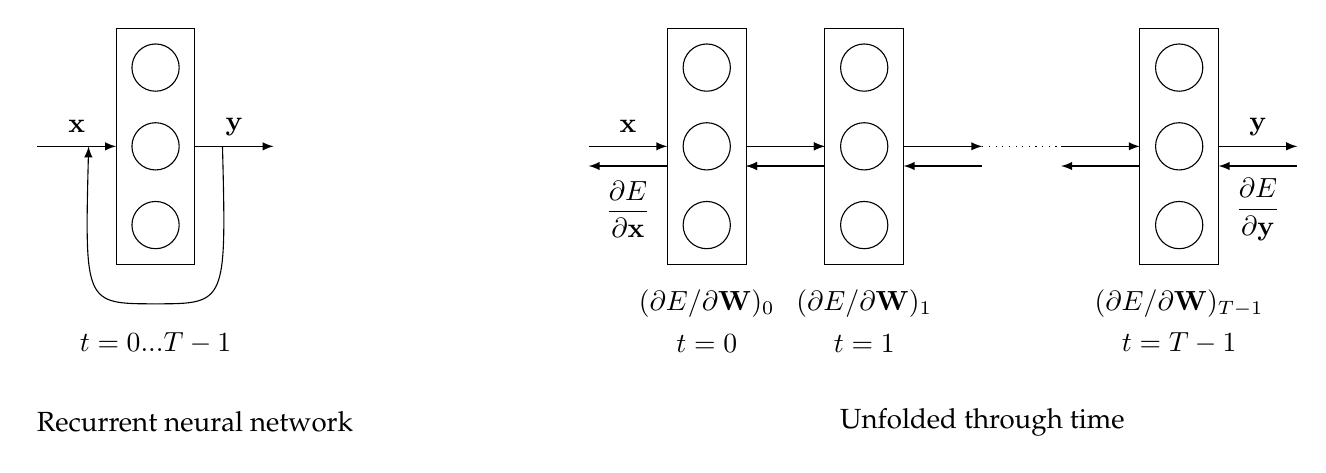
\begin{tikzpicture}
\draw (1.35,1.5) .. controls (1.4,-0.5) .. (0.5, -0.5);
\draw [latex-](-0.35,1.5) .. controls (-0.4,-0.5) .. (0.5, -0.5);
%\draw [-latex](1,1.5) .. controls (3, -1) and (-2, -1) .. (0,1.5);
\foreach \x in  {0, 7, 9, 13}
{
	\draw (\x,0) rectangle (\x+1,3);
	\draw (\x+0.5,2.5) circle (0.3cm);
	\draw (\x+0.5,1.5) circle (0.3cm);
	\draw (\x+0.5,0.5) circle (0.3cm);
	\draw [-latex](\x-1,1.5) -- (\x,1.5);
	\draw [-latex](\x+1,1.5) -- (\x+2,1.5);
}
\foreach \x in  {7, 9, 13}
{
	\draw [latex-](\x-1,1.25) -- (\x,1.25);
	\draw [latex-](\x+1,1.25) -- (\x+2,1.25);
}
\path (1, -2) node[draw=none] (left_title) {Recurrent neural network};
\path (11,-2) node[draw=none] (right_title) {Unfolded through time};
\path (0.5,-1) node[draw=none] (tA) {$t=0...T-1$};
\path (7.5,-1) node[draw=none] (t0) {$t=0$};
\path (9.5,-1) node[draw=none] (t1) {$t=1$};
\path (13.5,-1) node[draw=none] (tT1) {$t=T-1$};
\path (7.5,-0.5) node[draw=none] (t0) {$(\del E / \del \+W)_0$};
\path (9.5,-0.5) node[draw=none] (t1) {$(\del E / \del \+W)_1$};
\path (13.5,-0.5) node[draw=none] (tT1) {$(\del E / \del \+W)_{T-1}$};
\path (-0.5,1.75) node[draw=none] (Xleft) {$\+x$};
\path (1.5,1.75) node[draw=none] (Yleft) {$\+y$};
\path (6.5,1.75) node[draw=none] (Xleft) {$\+x$};
\path (14.5,1.75) node[draw=none] (Yleft) {$\+y$};
\path (6.5,0.7) node[draw=none] (Xleft) {$\dfrac{\del E}{\del \+x}$};
\path (14.5,0.7) node[draw=none] (Yleft) {$\dfrac{\del E}{\del \+y}$};
\draw [dotted] (11,1.5) -- (12,1.5);
\end{tikzpicture}
\caption{Back-propagation through time}
\label{fig:bptt}
\end{figure}

More RNN training techniques can be found in Appendix \ref{train_tech}.

\section {Word embedding}
In the previous sections, we have covered some neural network basics and popular configurations. In the following sections, we will introduce some recent applications in the field of natural language processing and question answering using word embeddings and recurrent neural networks.

A short definition for word embedding is a dictionary which assigns each vocabulary a high dimensional vector that captures semantic similarity. Typical English vocabulary size in NLP applications are between 10,000 and 100,000, and following the Zipf's law\cite{zipf49}, most of the vocabularies are rare words. In a typical n-gram analysis, our computational and storage resource quickly run out because of the sparsity of word combinations. To fight against this curse of dimensionality, one would like to share knowledge between similar words without redundant training examples for each word. For example in a language modelling task, if we have seen the sentence ``the cat is walking in the bedroom'', then the other sentence ``the dog was running in a room'' should also be assigned with higher probability \cite{bengio03}. While traditional non-parametric n-gram models fail to capture the associativity of similar words, neural networks have the ability to approximate the probability distribution over a continuous hyperspace. But to enable this task, we need to convert every word into its vector representation. We can first randomly initialize the word embedding matrix as the first layer of a neural network, and then train the network to predict the next word given a sequence of previous words. In the end, the first layer can be then used as a fine-tuned word embedding. The trained embedding vectors are distributed representation of words that preserve semantic similarity. Earlier word embeddings are mostly trained from neural language models, until recently researchers found that language modelling is not necessary to obtain a good word embedding.

\subsection{Skip-gram embedding model}
The skip-gram model \cite{mikolov13} is a very successful word embedding model. In the paper, the authors used two methods to train word vectors: the continuous bag of words (CBOW) and the skip gram model. The former aims to predict the missing word given a bag of context words, and the latter aims to predict the context surrounding a given single word. The model is streamlined to one single linear mapping which significantly shortens the training time down to a few minutes on a standard computer, as opposed to a few weeks for neural language models. It is also astonishing to see algebraic operators can be directly applied on word vectors, and can preserve the intended meaning. For example, ``king'' + 	``woman'' - ``man'' $\sim$ ``queen'' \cite{mikolov13}. The software package released with the paper is called ``word2vec.'' A lot of subsequent research directly uses this software to train general purpose or problem specific word embeddings.

\section{Jointly learn image and word}
Human beings are capable of associating objects of their different forms. For example, when people see a text ``pink pig'', they are likely to imagine a picture of a pink pig in their head. Likely, when people see blue sky in their eyes, they are likely to have some word-level mental activity. It is an intriguing question to ask if we can engineer a ``visual-semantic joint embedding,'' an abstract vector space in which the word ``sky'' and a picture of sky has very small distance. It is very tempting to build such an embedding on top of the existing convolutional neural networks and word embeddings. In the work ``Deep Visual-Semantic Embedding Model'' (DeViSE) \cite{frome13}, researchers used model proposed earlier \cite{weston10} but replaced the image feature extractors with the last hidden layer convolutional net \cite{krizhevsky12} (just before the softmax layer). The image representation is then mapped to the word embedding space \cite{mikolov13} with a linear transformation. The model is trained to correctly classify images, and the joint embedding outperforms the standard convolutional neural net by a large margin on a test set with a large number of unseen classes. The reason is that even though the exact images of the classes are unseen, the class names have already had their word similarity captured in the word embedding space, and thus beat the simple fully connected softmax layer in standard convolutional neural networks. Not only does joint embedding improves the result for image object recognition tasks, it also encourages better cooperation of visual and semantic knowledge. The work by \cite{kiros14b} proposed models that generate descriptions based on an image input using visual semantic embeddings, and the generated sentences have much better plausibility and accuracy compared to earlier results \cite{kulkarni11,mitchell12}. In their work, they used LSTM introduced earlier as part of the encoder of training descriptions as well as the decoder of generated descriptions. These recent works have shown us very strong feasibility to jointly learn image and text in a joint embedding space.

\section{Image-based question answering}
The following sections will focus on the background of question-answering and recent research specifically related to image-based question answering. Traditional QA builds entity relationships within a large text collection, or a corpus, using natural language processing (NLP) techniques. Large-scale question answering has a long history, mostly initiated via the Text Retrieval Conference (TREC). Despite some eminent successes in building such systems, such as \cite{lewis12}, building a knowledge graph requires a great amount of engineering and is heavily dependent on the knowledge base or the search engine, and is also hard to generalize to unseen entities. There have been ongoing efforts of using embedding-based model and recurrent neural networks on question-answering tasks. \cite{weston14} showed that their memory-based recurrent neural network can perfectly answer questions that involve long time dependency in a paragraph.

Image-based question answering has its own differences compare to text-based question answering:
First, the question is centered on the image. Therefore, the model needs to acquire both visual and semantic knowledge.
Second, unlike traditional question answering where the training data contains almost the exact answer with certain predicates revealing its relation with the question, here the training data provides no direct information to the answer, which is solely contained the unseen test image. However, the training data provides very strong clue of what catagories of answers are expected. For example, the model should be able to conclude from the training data that ``chair'' is a more probable answer than ``window'' for a question like ``What is around the table?''  These differences actually make the problem unique from traditional QA tasks.

\subsection{DAQUAR dataset}
\label{background_daquar}
In 2014, Malinowski et al. released a dataset with images and question-answer pairs. It is called DAtaset for QUestion Answering on Real-world images (DAQUAR) \cite{malinowski14a}. All images are from the NYU depth v2 dataset \cite{silberman12}, and are taken from indoor scenes. Human segmentations, image depth values, and object labellings are available in the dataset. The QA pairs were created by human crowdsourcing. The original train-test split ratio is about 3800:3300. The QA data has two sets of configuration: the 37-class and the 894-class dataset, differed by the number of object classes appearing in the questions. There are mainly three types of questions in this dataset:
\begin{enumerate}
	\item Object type
	\item Object colour
	\item Number of objects
\end{enumerate}
Qualitatively speaking, a large proportion of the questions are very hard to answer. Figure~\ref{fig:difficult} summarizes the sources of difficulties. Since DAQUAR is the only publicly available image-based QA dataset, it is one of our benchmarks to evaluate our models.

\begin{figure}
    \centering
    \footnotesize
    \begin{subfigure}[t]{0.3\textwidth}
            \includegraphics[width=\textwidth]{red.jpg}
            Q7: what colour is the ornamental plant in fornt of the fan coil but not close to sofa ? -red
            \caption{Hard to locate the object}
    \end{subfigure}%
    \quad
    \begin{subfigure}[t]{0.3\textwidth}
            \includegraphics[width=\textwidth]{black.jpg}
            Q20: how many black objects are on the desk ? -three
            \caption{Counting ambiguity, could be three to five}
    \end{subfigure}
    \quad
    \begin{subfigure}[t]{0.3\textwidth}
            \includegraphics[width=\textwidth]{blind.jpg}
            Q1129: what is behind the tap ? -blinds
            \caption{Object ambiguity, could be a window or blinds}
    \end{subfigure}
    \quad
    \begin{subfigure}[t]{0.3\textwidth}
            \includegraphics[width=\textwidth]{sink.jpg}
            Q5: what is under the white cabinet on the right side of the oven and and on the left side of the fridge ? -sink
            \caption{Lengthy description of spatial relations}
    \end{subfigure}
    \quad
    \begin{subfigure}[t]{0.3\textwidth}
            \includegraphics[width=\textwidth]{brown.jpg}
            Q1423: what is the colour of the furniture ? -brown
            \caption{Colour ambiguity due to dim lighting}
    \end{subfigure}
    \quad
    \begin{subfigure}[t]{0.3\textwidth}
            \includegraphics[width=\textwidth]{paper.jpg}
            Q1467: what is on the night stand ? -paper
            \caption{Object is too small}
    \end{subfigure}
    \caption{Various types of difficult questions in the DAQUAR dataset}
	\label{fig:difficult}
\end{figure}

\subsection{Previous attempt}
Together with the release of the DAQUAR dataset, \cite{malinowski14b} presented an approach which combines semantic parsing and image segmentation. In the natural language part of their work, they used a semantic parser \cite{liang13} to convert sentences into latent logical forms. The parser is specially designed for QA tasks, and can be trained well where the true dependency tree is missing from the training data. In the image part, they evaluated different latent logical forms of the question with multiple segmentation. They obtained the multiple segmentations of the image by sampling the uncertainty of the segmentation algorithm. Their model is based on a Bayesian formulation that every logical form and image segmentation has certain probability. To make the inference step of their algorithm scalable, they chose to sample from the nearest neighbours in the training set according to the similarity of the semantic parsing.

While their model seems to handle a number of spatial relations, their predefined set of possible predicates constrains the question form and the environment. Moreover, the quality of answers also depends on the accuracy of the automatic image segmentation algorithm. Lastly, inferring all possible predicates between every pair of objects does not scale to larger dataset. The embedding space models introduced earlier have significant differences with their approach, and we hope that our embedding space model will outperform their model in terms of answer accuracy and similarity.
\chapter{Methods and Results}
\section{Problem restatement}
We consider every examples in a image QA dataset as a triplet of an image vector, a question of a sequence of word indices, and an answer of a sequence of word indices. We start off by assuming that the answers are all one-word answers, i.e. the length of the answer sequence is always one. The assumption is established based on more than 98\% of the data entries in DAQUAR have only one-word answers. Our goal is to learn a function that takes the input of an image vector and a sequence of word indices, and emits the output of the answer word. 

\section{Our models}
\subsection{GUESS model}
One very simple baseline is to predict the mode based on question type. For example, if the question contains ``how many'' then output ``two.'' This baseline actually works unexpectedly well in DAQUAR dataset.

\subsection{BOW model}
Another baseline is to use the last hidden layer of the Oxford convolutional neural net (4096 dimension) \cite{simonyan14} as an image feature extractor, and use wording embeddings from word2vec. To obtain the sentence-level embedding, we simply sum all the word vectors, i.e. bag-of-words (BOW). We concatenate the image vectors and the word vectors, and send the combined feature into a softmax layer.

\subsection{LSTM sentence model}
Due to the sequential nature of natural languages, researchers have been looking for ways to model sentences using recurrent neural networks. There has been increasing interests in using LSTM to model the embedding vector for a whole sentence. Recently, \cite{sutskever14} uses LSTM as both encoders and decoders in machine translation, and achieved BLEU score \cite{bleu} better than the traditional phrase-based models \cite{luong14}. In our work we use LSTM as our sentence embedding model. At every timestep we input a word vector to the LSTM, and we use the output values of the LSTM at the last timestep as our embedding space representation of the question asked.

\subsection{Image-word model}
We started off the experiment by directly building on top of the LSTM sentence model. In this experiment, we designed a model called the ``image-word model'' because it treats the image as one word of the question. We borrowed the idea of treating the image as the first word of the question from caption generation by \cite{vinyals14}. The difference with caption generation is that here we only output the answer at the last time step.

\begin{enumerate}
	\item We used the last hidden layer of the Oxford convolutional neural net (4096 dimension) \cite{simonyan14} as our visual embedding model.
	\item We use the word2vec embedding model (skip gram) trained from Google News \cite{mikolov13} as our frozen semantic embedding (300 dimension). 
	\item We then treated the image as if it is the first word of the sentence. In order to map the image embedding to our semantic embedding space, we used a linear transformation layer of dimension 4096$\times$300 (similar to \cite{frome13}).
	\item The last time step of the LSTM output is passed to a softmax layer. The final output is a 68-dimension vector representing the probability of the answer being each possible answer classes.
\end{enumerate}

We used the 37 class DAQUAR dataset, so the question and answers will only focus on 37 object classes. We also filtered dataset down to only one-word answers. This simplification trims the possible set of answers to 63 words (including unknown class ``UNK'').
To evaluate the model, we used the plain answer accuracy as well as the Wu-Palmer similarity (WUPS) measure \cite{wu94, malinowski14b}. The WUPS calculates the similarity between two words based on their longest common subsequence in the taxonomy tree. The similarity function takes in a threshold parameter. If the similarity between two words is less than the threshold then zero score will be given to the candidate answer. It reduces to plain accuracy when the threshold equals to 1.0. Following \cite{malinowski14b}, we measure all the models in terms of plain accuracy, WUPS at 0.9 threshold, and WUPS at 0.0 threshold.

To evaluate the results, we also designed a baseline model to avoid over-interpretation. In this model, the images are replaced by randomly generated vectors instead of meaningful graphics. We call this baseline the ``blind model.''

\begin{figure}
\centering
\scalebox{0.9}{
\input{imgword.tex}}
\caption{Image-word model and blind model}
\label{fig:imgword}
\end{figure}

\subsection{Bidirectional image-word model}
The image-word model, which takes in words sequentially in a linear fashion, may not be powerful enough to handle complex sentence structures in the question. At the last timestep it needs to output the answer immediately after reading the last word of the question. In some cases where the hint is revealed at the last timestep, the single direction model may fail to change direction because the previous words have made the model very confident of an answer already. The bidirectional image-word model aims to fix this weakness. It contains two LSTMs. The first one takes the image as the first word and then processes the words sequentially just like the previous model. Moreover, the second LSTM processes the words in a reverse order, together with the hidden state of the first LSTM at that timestep. At the last timestep, the second LSTM takes in the image again. So intuitively, the first timestep gives an ``impression'' of the image, and after knowing the sentence, it checks the image again to confirm the answer. The second LSTM ``sees'' the whole sentence at every timestep, so this model is thought to be better because it considers the entire question for a longer period of time.

\begin{figure}[h]
\centering
\scalebox{0.9}{
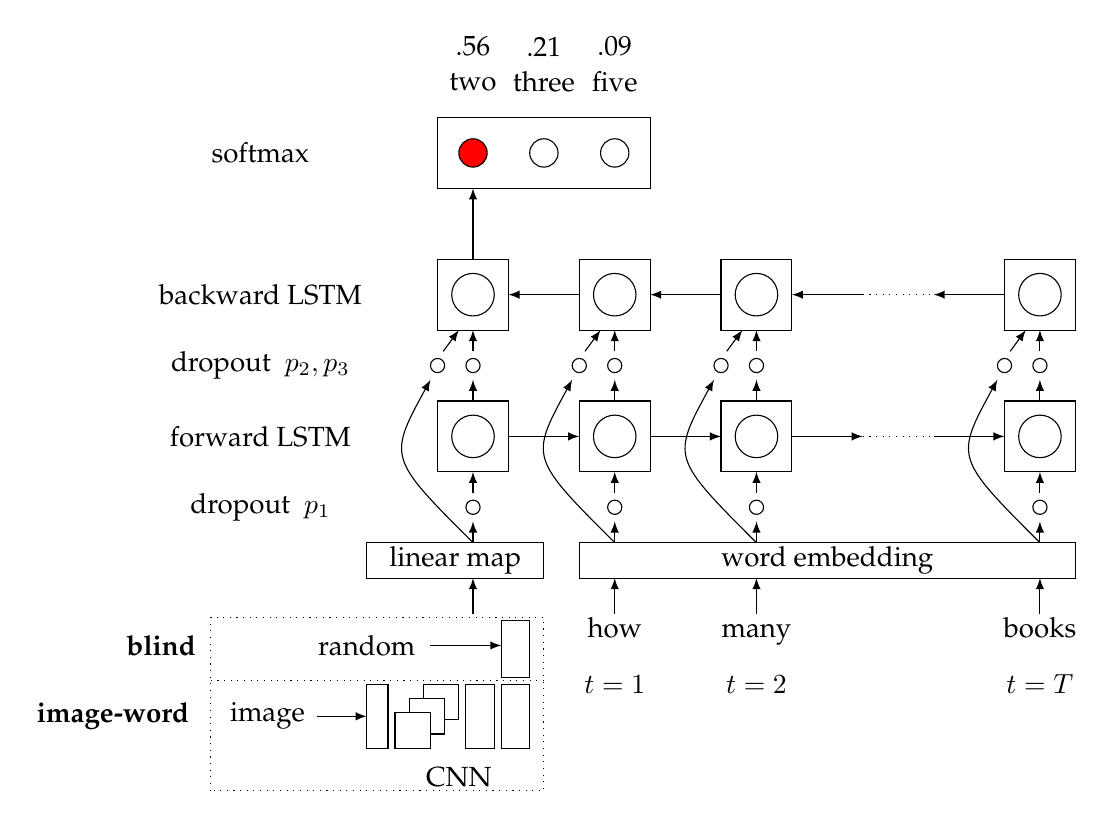
\begin{tikzpicture}[scale=0.9]

\foreach \x in  {5, 7, 9, 13}
{
    \draw (\x,3.0) rectangle (\x+1,4.0);
    \draw (\x+0.5,3.5) circle (0.3cm);
    \draw [-latex](\x+0.5,2.0) -- (\x+0.5,2.3);
    \draw (\x+0.5,2.5) circle (0.1cm);
    \draw (\x-0.0,2.5) circle (0.1cm);
    \draw [-latex](\x+0.5,2.7) -- (\x+0.5,3.0);
}

\foreach \x in  {7, 9, 11, 13}
{
    \draw [latex-](\x-1,3.5) -- (\x,3.5);
}
\draw [dotted] (11,3.5) -- (12,3.5);


\foreach \x in {5.5, 7.5, 9.5, 13.5}
{
    \draw [-latex](\x, 0.0) .. controls (\x-1.2,1.2) .. (\x-0.6,2.3);
    \draw [-latex](\x-0.42, 2.7) -- (\x-0.2, 3.0);
}

\foreach \x in  {5, 7, 9, 13}
{
    \draw (\x,1) rectangle (\x+1,2);
    \draw (\x+0.5,1.5) circle (0.3cm);
    \draw [-latex](\x+0.5,0) -- (\x+0.5,0.3);
    \draw (\x+0.5,0.5) circle (0.1cm);
    \draw [-latex](\x+0.5,0.7) -- (\x+0.5,1);
}

\foreach \x in  {7, 9, 13}
{
    \draw [-latex](\x+0.5,-1) -- (\x+0.5,-0.5);
}

\foreach \x in  {7, 9, 11, 13}
{
    \draw [-latex](\x-1,1.5) -- (\x,1.5);
}

\path (7.5,-2) node[draw=none] (t0) {$t=1$};
\path (9.5,-2) node[draw=none] (t1) {$t=2$};
\path (13.5,-2) node[draw=none] (tT1) {$t=T$};
\draw [dotted] (11,1.5) -- (12,1.5);

\path (7.5,-1.2) node[draw=none] (w1) {how};
\path (9.5,-1.3) node[draw=none] (w2) {many};
\path (13.5,-1.2) node[draw=none] (w3) {books};
\path (2.5,0.5) node[draw=none] (drop) {dropout $~p_1$};
\path (2.5,1.5) node[draw=none] (lstm1) {forward LSTM};
\path (2.5,2.5) node[draw=none] (drop) {dropout $~p_2, p_3$};
\path (2.5,3.5) node[draw=none] (lstm1) {backward LSTM};
\draw (7, -0.5) rectangle (14, 0);

\draw (5,5) rectangle (8,6);
\draw[fill=red] (5.5,5.5) circle (0.2cm);
\draw (6.5,5.5) circle (0.2cm);
\draw (7.5,5.5) circle (0.2cm);
\path (2.5,5.5) node[draw=none] (logit) {softmax};
\path (5.5,6.5) node[draw=none] (logit2) {two};
\path (6.5,6.5) node[draw=none] (logit3) {three};
\path (7.5,6.5) node[draw=none] (logit5) {five};
\path (5.5,7) node[draw=none] (logit2) {.56};
\path (6.5,7) node[draw=none] (logit3) {.21};
\path (7.5,7) node[draw=none] (logit5) {.09};
\draw [-latex] (5.5,4) -- (5.5,5);

\draw (4,-0.5) rectangle (6.5, 0);
\path (5.25,-0.25) node[draw=none] (imgMap) {linear map};

\draw (4.0, -2.9) rectangle (4.3, -2);
\draw[fill=white] (4.8, -2.5) rectangle (5.3, -2);
\draw[fill=white] (4.6, -2.7) rectangle (5.1, -2.2);
\draw[fill=white] (4.4, -2.9) rectangle (4.9, -2.4);
\draw (5.4, -2.9) rectangle (5.8, -2);
\draw (5.9, -2.9) rectangle (6.3, -2);
\draw (5.9, -1.9) rectangle (6.3, -1.1);
\draw [-latex] (5.5, -1.0) -- (5.5, -0.5);

\draw [-latex] (4.9,-1.45) -- (5.9, -1.45);
\draw [-latex] (3.3,-2.45) -- (4.0, -2.45);
\path (4.0,-1.45) node[draw=none] (random) {random};
\path (2.6,-2.45) node[draw=none] (image) {image};
\path (1.1,-1.45) node[draw=none] (blind) {\textbf{blind}};
\path (0.42,-2.45) node[draw=none] (image-word) {\textbf{image-word}};
\path (5.3,-3.3) node[draw=none] (cnn) {CNN};
\draw [dotted] (1.8,-1.95) -- (6.5, -1.95);
\draw [dotted] (1.8,-3.5) rectangle (6.5, -1.05);

\path (10.5,-0.25) node[draw=none] (Wemb) {word embedding};


\end{tikzpicture}}
\caption{Bidirectional image-word model and blind model}
\label{fig:imgword}
\end{figure}

\subsection{Image-word ranking model}
The softmax layer can be replaced by other types of loss. The ranking loss is very popular in recent question answering literature because it is very fast to train. This type of model outputs a vector that is the nearest neighbour of the answer word in the semantic embedding. The error function uses the pair-wise ranking loss \cite{weston10}, defined below:

\begin{equation}
\sum\limits_{\+y} \sum\limits_{i \neq j} \max \{0, \alpha-s(\+y, \+a_j) + s(\+y, \+a_i) \}
\end{equation}

$\+y$ and $\+a$ are both vectors in the answer embedding space. $\+y$ is the output of the model, and $\+a_j$ is the correct answer for the question, and $\+a_i$ is one of any possible answers. $s(\cdot, \cdot)$ denotes the similarity measure of two vectors. It is usually implemented as the cosine similarity in high dimensional spaces: 
\begin{equation}
s(\+x, \+y) = \dfrac{\+x \cdot \+y} {\norm{\+x} \norm{\+y}}
\end{equation}

This error function will penalize the model if the right answer is not winning over other wrong answers by a certain margin $\alpha$. It is a widely used in ranking image descriptions \cite{kiros14b}. The ranking loss effectively replaces the softmax layer, and the hidden dimension of the LSTM need to match with the word embedding dimension. 

\subsection{DAQUAR results}
\label{sec:daquar_results}
Table~\ref{tab:daquar_results} summarizes the performance of our proposed models and our baselines. First, our models win by a large margin compared to the results from the publisher of the DAQUAR dataset. Second, we argue that most gain in accuracy results from a good sentence embedding, because the blind model has almost the same accuracy compared to the image-word model. Third, the bidirectional model further improves the performance by a small amount. Lastly, the ranking loss model does not outperform the softmax model. Although the training is much faster even with a smaller learning rate, it achieves lower accuracy because it tends to overfit the training set too quickly.

In Figure~\ref{fig:imgword+blind}, we further discovered the some weak visual ability by a direct comparison of test examples. We observed that the image-word model seems to perform better on questions centered on dominant objects or dominant colours, but does not seem to learn how to count.

\begin{figure}
    \centering
    \footnotesize
    \begin{subfigure}[t]{0.3\textwidth}
            \includegraphics[width=\textwidth]{bed_vs_table.jpg}
            Q193: what is the largest object ?\\
            Image-word: table (0.576)\\
            Blind: bed (0.440)\\
            Ground truth: table
            \caption{The question gives no extra clue of the class of the object. The visual model recognizes the correct object through the shape.}
    \end{subfigure}%
    \quad
    \begin{subfigure}[t]{0.3\textwidth}
            \includegraphics[width=\textwidth]{fridge_vs_toilet.jpg}
            Q212: what is the object left of the room divider ?\\
            Image-word: toilet (0.3973), sink (0.1367), towel (0.1323)\\
            Blind: refridgerator (0.5318)\\
            Ground truth: door
            \caption{The visual model recognizes the correct scene.}
    \end{subfigure}
    \quad
    \begin{subfigure}[t]{0.3\textwidth}
            \includegraphics[width=\textwidth]{three_vs_three.jpg}
            Q1615: how many pictures are there on the wall ?\\
            Image-word: three (0.4518)\\
            Blind: three (0.6047)\\
            Ground truth: seven
            \caption{No evidence shows that image-word model learns how to count.}
    \end{subfigure}
    \caption{Direct comparison between the image-word model and the blind model.}
    \label{fig:imgword+blind}
\end{figure}

\begin{table}[h]
\centering
\caption{DAQUAR results}
\label{tab:daquar_results}
\begin{minipage}{10.5cm}
%{6cm}
\begin{tabular}{l l l l l l l l}
\toprule
                 & \textbf{Accuracy} & \textbf{WUPS 0.9} & \textbf{WUPS 0.0}\\
\midrule
\textbf{2-IMGWD}\footnote{Bidirectional image-word model} & \textbf{0.3276} & \textbf{0.3298} & 0.7272\\
\textbf{IMGWD}\footnote{Image-word model}   & 0.3188   & 0.3211 & \textbf{0.7279}\\
\textbf{IMGWD-RK}\footnote{Image-word ranking model}   & 0.2787 & 0.2782 & 0.7074\\
\midrule
\textbf{BLIND}\footnote{Single-direction blind model}   & 0.3051   & 0.3069 & 0.7229\\
\textbf{RANDWD}\footnote{Single-direction model with random word embedding}  & 0.3036   & 0.3056 & 0.7206\\
\textbf{BOW}\footnote{Bag-of-words model}     &  0.2299  & 0.2340 & 0.6907\\
\textbf{GUESS}\footnote{Guess ``two'', ``white'', and ``table'', depending on question type}   & 0.1785   & 0.1823       & 0.6874\\
\textbf{MultiWorld \cite{malinowski14b}} & 0.1273 & 0.1810 & 0.5147\\
\midrule
\textbf{HUMAN} & 0.6027 & 0.6104 & 0.7896\\
\bottomrule
\end{tabular}
\end{minipage}
\end{table}

\section{COCO-QA dataset}
From DAQUAR results, we see that although our models have improved the answer accuracy by a lot compared to the previous attempt, the blind version of the model can do almost equally well, suggesting that the image features from the CNN are not very useful. Since 1500 images are a very small dataset, maybe it is worthwhile for us to build a larger dataset so that the neural networks can be trained more robustly.

Manually annotating pictures with QA pairs requires large amount of time, capital, and tools. We propose to use currently massively available image description dataset and convert descriptions into QA forms. This method is cheap, fast, and scalable; however the drawback is that the quality of automatically generated questions is unforeseeable. There lacks a measure to test how sensical the questions are overall.

We used recently released Microsoft Common Objects in COntext (MS-COCO) \cite{mscoco} dataset, which contains 100K images and 500K sentence descriptions, and converted the descriptions into QA pairs. We only considered three types of questions: object, number, and colour, and only single-word answers.

\subsection{Question conversion algorithms}
Here we present an algorithm that converts sentences into different types of questions.

\subsubsection{Object-type questions}
First, we consider asking an object using ``what'' or ``who''. This involves replacing the actual object with a ``what'' in the sentence, and then transforming the sentence structure so that the ``what'' appears in the front of the sentence. The algorithm below assumes that the input is a sentence in the form of a syntactic tree, and the output is a question in the form of a syntactic tree.

The entire algorithm has the following stages:
\begin{enumerate}
\item Split long sentences into simple sentences (see Algorithm~\ref{alg:splitcc}). \\
For question generation task, sentences need not to be very descriptive, and shorter the original sentences are, more readable the questions will be. Moreover, the wh-words that are found in sub-sentences or clauses will less likely be able to perform wh-movement \cite{borsley99}. Here we only consider a simple case that is when two sentences are joined together with a conjunctive word ``and''. We split the orginial sentences into two independent sentences.
 For example, ``There is a cat and the cat is running.'' will be split as ``There is a cat.'' and ``The cat is running.''
\item Change indefinite determiners to definite determiners (see Algorithm~\ref{alg:indef2def}).\\
Asking questions on a specific instance of the subject requires changing the determiner into definite form ``the''. For example, ``\textbf{A} boy is playing \underline{baseball}.'' will have ``the'' instead of ``a'' in its question form: ``\underline{What} is \textbf{the} boy playing?''.

\item Traverse the sentence and identify potential answers (see Algorithm \ref{alg:traverseWhat}). \\
We traverse the tree structure and identify answers that belong to certain word categories. Then we replace the answer with a question word ``what'' or ``who'' depending on the object type.

\item Perform wh-movement with some constraints (see Algorithm~\ref{alg:whmove}). \\
For English language, questions tend to start with interrogative words such as ``what'' and ``who''. The algorithm needs to move the verb as well as the ``wh-'' constituent to the front of the sentence. However, not all sentences allow such transformation. In this work we consider the following constraints:
\begin{enumerate}
\item A-over-A principle\\
The A-over-A principle was first discovered by Chomsky \cite{chomsky73}. For example, ``I am talking to John and \textbf{Bill}'' cannot be transformed into ``*Who am I talking to John and'' because ``Bill'' is an noun phrase (NP) constituent that is under another NP ``John and Bill''. Therefore, the child NP cannot be removed from the parent NP in the wh-movement.
\item Clauses\\
Except for a few cases, interrogative words in clauses usually cannot be moved to the front of the sentences. For example, ``I am riding a motorcycle that \textbf{Bill} wanted.'' cannot be transformed into ``*Who am I riding a motorcycle that wanted.''. In the future, there is a need to separate the original sentences into two: ``I am riding a motorcycle.'' and ``Bill wanted the motorcycle.''. For now, wh-word in the clauses will terminate the wh-movement process and our algorithm will only output sentences like ``I am riding a motorcycle that \textbf{who} wanted?''.
\end{enumerate}
\end{enumerate}

The entry point of the overall algorithm is shown in Algorithm~\ref{alg:askWhat}. Figure~\ref{fig:whmove} illustrates these procedures with tree diagrams. We used WordNet \cite{wordnet} and NLTK software package \cite{nltk} to lemmatize verbs and to get noun categories. We used Stanford parser \cite{klein03} to obtain syntatic structure of the original sentence.
\begin{algorithm}
\caption{Split compound sentences}
\label{alg:splitcc}
\begin{algorithmic}[1]
\Require Root of the syntactic tree of the original sentence
\Ensure List of roots of syntactic trees of split sentences
\Procedure{SplitCC}{root}
\State node $\gets$ root.children$[0]$ \Comment{Search directly from ``S'' node}
\If{node is ``S'' and it has more than 3 children}
    \If{All children are ``S'' or ``CC'' and ``CC''s are always in between two ``S''s}
        \State \Return each ``S'' child
    \EndIf
\EndIf
\EndProcedure
\end{algorithmic}
\end{algorithm}

\begin{algorithm}
\caption{Replace indefinite determiners to definite determiners}
\label{alg:indef2def}
\begin{algorithmic}[1]
\Require Root of the syntactic tree with wh-word in the original place
\Ensure Root of the syntactive tree with wh-word in the front
\Procedure{SwitchDefDet}{root}
\State node $\gets$ \Call{DFS}{root, ``NP''} \Comment{Depth-first search for the subject in the sentence}
\State node $\gets$ \Call{DFS}{node, ``DT''} \Comment{Depth-first search for the determiner of the subject}
\If{node.text = ``a'' \textbf{or} node.text = ``an''}
    \State node.text $\gets$ ``the''
\EndIf
\State \Return root
\EndProcedure
\end{algorithmic}
\end{algorithm}

\begin{algorithm}
\caption{Identify object-type answers}
\label{alg:traverseWhat}
\begin{algorithmic}[1]
\Require Root of the syntactic tree of the original sentence
\Ensure List of roots of the syntactic trees with answers replaced by ``what''
\Procedure{TraverseWhat}{root, results}
\For{child $\in$ node.children}
    \State \Call{TraverseWhat}{child, results}
\EndFor
\If{node is``NP'' and node's children contains a noun is of category\\
    \hspace{\algorithmicindent} \hspace{\algorithmicindent} animal, artifact, body, food, object, plant, possession, shape, person}
    \State answer $\gets$ noun
    \State whatNode $\gets$ Node(class=``WP'', text=``who/what'', children=$[\ ]$)
    \State Replace answer with Node(class=``WHNP'', text=``'',  children=$[$whatNode$]$)
    \State Insert the modified root into roots list
\EndIf
\EndProcedure
\end{algorithmic}
\end{algorithm}

\begin{algorithm}
\caption{Wh-movement}
\label{alg:whmove}
\begin{algorithmic}[1]
\Require Root of the syntactic tree with wh-word in the original place
\Ensure Root of the syntactive tree with wh-word in the front
\Procedure{Wh-movement}{root}

\State Check if the sentence contains a verb-phrase. If no, terminate.
\State Check if ``WHNP'' is under ``SBAR'' or ``NP''. If yes, terminate.

\State verbFront $\gets$ \textbf{null}
\If{the verb is any tensed form of ``be'' or ``have done'', or is a modifier e.g. ``will''}
    \State verbFront $\gets$ verb
    \State Remove verb from its parent
\Else
    \State verbFront $\gets$ Node(class=verb.class, text=``does/do/did'', children=$[]$)
    \State verb $\gets$ \Call{Lemmatize}{verb}
\EndIf

\State Remove WHNP from its parent
\State S\_old $\gets$ root.children$[0]$
\State S\_old.children.insert(verbFront, 0) \Comment{Insert verbFront as the first child of S\_old}
\State S\_new $\gets$ Node(class=``S'', text=``'', children=$[$WHNP, S\_old$]$)
\State root.children $\gets [$S\_new$]$
\State \Return root
\EndProcedure
\end{algorithmic}
\end{algorithm}

\begin{algorithm}
\caption{Generate object-type questions}
\label{alg:askWhat}
\begin{algorithmic}[1]
\Require Root of the syntactic tree of the original sentence
\Ensure List of roots of the syntactic trees of generated questions

\Procedure{AskWhat}{Root}
\State \Call{SwitchDefDet}{root}
\For {r $\in$ \Call{SplitCC}{root}}
    \State roots $\gets [\ ]$, \Call{TraverseWhat}{r, roots}
    \For {r2 $\in$ roots}
        \State \textbf{yield return} \Call{Wh-movement}{r2}
    \EndFor
\EndFor
\EndProcedure
\end{algorithmic}
\end{algorithm}


\begin{figure}[h]
    \centering
    \small
    \begin{subfigure}[t]{0.45\textwidth}
        \caption{Step 1: Parse the sytactic structure.}
        \centering
        \scalebox{0.8}{
        \Tree [.S [.NP [.DET a ] [.N man ] ] [.VP [.V is ] [.NP [.VBG riding ] [.NP [.DET a ] [.N horse ] ] ] ] ]}
        \vspace{5mm}
    \end{subfigure}
    \quad
    \begin{subfigure}[t]{0.45\textwidth}
        \caption{Step 2: Change determiner.}
        \centering
        \scalebox{0.8}{
        \Tree [.S [.NP [.DET \textbf{the} ] [.N man ] ] [.VP [.V is ] [.NP [.VBG riding ] [.NP [.DET a ] [.N horse ] ] ] ] ]}
        
        \vspace{5mm}
    \end{subfigure}
    \begin{subfigure}[t]{0.45\textwidth}
        \caption{Step 3: Find the answer of the question.}
        \centering
        \scalebox{0.8}{
        \Tree [.S [.NP [.DET the ] [.N man ] ] [.VP [.V is ] [.NP [.VBG riding ] [.NP [.DET \textbf{a} ] [.N \textbf{horse} ] ] ] ] ]}
        \vspace{5mm}
    \end{subfigure}
    \quad
    \begin{subfigure}[t]{0.45\textwidth}
        \caption{Step 4: Replace the answer with ``what''.}
        \centering
        \scalebox{0.8}{
        \Tree [.S [.NP [.DET the ] [.N man ] ] [.VP [.V is ] [.NP [.VBG riding ] [.NP [.DET \sout{a} ] [.N \sout{horse} ] ] ] ] ]}
        \vspace{5mm}
    \end{subfigure}
    \begin{subfigure}[t]{0.45\textwidth}
        \caption{Step 4: Replace the answer with ``what''.}
        \centering
        \scalebox{0.8}{
        \Tree [.S [.NP [.DET the ] [.N man ] ] [.VP [.V is ] [.NP [.VBG riding ] [.WHNP [.WP \textbf{what} ] ] ] ] ]}
        \vspace{5mm}
    \end{subfigure}
    \quad
    \begin{subfigure}[t]{0.45\textwidth}
        \caption{Step 5: Perform WH-fronting.}
        \centering
        \scalebox{0.8}{
        \Tree [.S [.WHNP [.WP what ] ] [.S [.V is ] [.NP [.DET the ] [.N man ] ] [.VP [.V \sout{is} ] [.NP [.VBG riding ] [.WHNP [.WP \sout{what} ] ] ] ] ] ]}
        \vspace{5mm}
    \end{subfigure}
    \caption{
        Example: ``A man is riding a \textbf{horse}'' $=>$ ``\textbf{What} is \textbf{the} man riding?''}
    \label{fig:whmove}
\end{figure}

\subsubsection{Number-type questions}
To generate ``how many'' types of questions, we follow a similar procedure as the previous algorithms, except a different way to identify potential answers. This time, we need to extract numbers from original sentences. Splitting compound sentences, changing determiners, and wh-movement parts remain the same. Algorithm~\ref{alg:traverseHowMany}, \ref{alg:askHowMany} shows an detailed algorithm.

\begin{algorithm}[h]
\caption{Identify number-type answers}
\label{alg:traverseHowMany}
\begin{algorithmic}[1]
\Require Root of the syntactic tree of the original sentence
\Ensure List of roots of the syntactic trees with answers replaced by ``how many''
\Procedure{TraverseHowMany}{root, results}
\For{child $\in$ node.children}
    \State \Call{TraverseHowMany}{child, results}
\EndFor
\State answer $\gets$ \textbf{null}
\If{node is ``NP'' and node's children contains number}
    \State howNode $\gets$ Node(class=``WRB'', text=``how'', children=$[\ ]$)
    \State manyNode $\gets$ Node(class=``JJ'', text=``many'', children=$[\ ]$)
    \State parent $\gets$ Node(class=``WHNP'', text=``'', children=$[$howNode, manyNode$]$)
    \State Replace the number node with parent
    \State Insert the modified root into results list
\EndIf
\EndProcedure
\end{algorithmic}
\end{algorithm}

\begin{algorithm}[h]
\caption{Generate number-type questions}
\label{alg:askHowMany}
\begin{algorithmic}[1]
\Require Root of the syntactic tree of the original sentence
\Ensure List of roots of the syntactic trees of generated questions

\Procedure{AskHowMany}{Root}
\State results $\gets [\ ]$
\State \Call{SwitchDefDet}{root}
\For {r $\in$ \Call{SplitCC}{root}}
    \State roots $\gets [\ ]$, \Call{TraverseHowMany}{r, roots}
    \For {r2 $\in$ roots}
        \State \textbf{yield return} \Call{Wh-movement}{r2}
    \EndFor
\EndFor
\EndProcedure
\end{algorithmic}
\end{algorithm}

\subsubsection{Colour-type questions}
Compared to the previous two question types, colour-type questions are much easier to generate. It only requires locating the colour adjective and the noun which the adjective attaches to. Then it simply forms a sentence ``What is the colour of the object'' with the ``object'' replaced by the actual noun. The tree traversal is also similar to previously presented algorithms so the implementation details are omitted.

\subsection{Reducing rare answers}
Here we impose a hard constraint such that all answers must at least appear $L$ times in the dataset. In the 6.6K dataset, $L=5$, and in the full dataset, $L=20$. The reason of imposing this constraint is that otherwise we would end up with many answers that only appear once in the training set. This will significantly increase the difficulty of the task.

\subsection{Reducing common answers}
Besides creating more data, the other main motivation here is to reduce the performance of a model that simply guesses for the three most common answers (i.e. mode guessing) for each type of question (e.g. ``man'', ``two'', ``white''). Therefore, additional constraint needs to be imposed to reduce the common answers. The probability of enrolling an question-answer pair $(q, a)$ is:
\begin{equation}
p(q, a) = \left\{ \begin{array}{cl}
1 &\mbox{ if \text{count}$(a)$ $\le U$ } \\
\exp\left(-\dfrac{\text{count}(a) - U}{2U}\right) &\mbox{ otherwise }
\end{array} \right.
\end{equation}
where $U=100$ in both the 6.6K dataset and the full dataset. This will penalize answers for appearing more than $U$ times while still preserve the rank of the most common answers.

\subsection{Question statistics}
With the automatic question generation technique described above, we gathered a dataset from the MS-COCO dataset. We name this dataset to be COCO-QA dataset. Table~\ref{tab:cocoqa_stats} presents some important statistics of COCO-QA, with comparison to DAQUAR. The full dataset is considered to be harder than DAQUAR, because it has more possible answer classes and lower guess baseline accuracy. However, COCO-QA contains 60 times more images and 20 times more question-answer pairs, so it is more suitable to deep learning approaches.

\begin{table}[h]
\centering
\caption{General statistics of COCO-QA and DAQUAR}
\label{tab:cocoqa_stats}
\begin{minipage}{14cm}
\begin{tabular}{c c c c c}
\toprule
\textbf{Dataset} & \textbf{\# Images} & \textbf{\# Questions} & \textbf{\# Answers\footnote{Number of answers present in the training set plus the unknown ``UNK'' class}} & \textbf{GUESS accuracy}\footnote{Guess the three most common answers depending on question types}\\
\midrule
DAQUAR-37\footnote{Trimmed to include only single-word answer}  &  795+654\footnote{``+'' denotes train-test split}  & 3825+3284  & 63     & 0.1885\\
DAQUAR-894\footnote{Trimmed to include only single-word answer}  &  795+654  & 6149+5076  & 412    & 0.1180\\
COCO-QA 6.6K & 3.6K+3K      & 14K+11.6K  & 298        & 0.1157         \\
COCO-QA Full & 80K+20K      & 177K+83K & 794           & 0.0347\\
\bottomrule
\end{tabular}
\end{minipage}
\end{table}

\begin{table}[h]
\centering
\caption{
COCO-QA and DAQUAR question type break-down (numbers inside the brackets denote the proportion with regard to the entire dataset)}
\begin{tabular}{c c c c c c}
\toprule
\textbf{Dataset}      &         & \textbf{Object} & \textbf{Number} & \textbf{Colour} & \textbf{Total}  \\
\midrule
\textbf{DAQUAR-37}    & Train   & 2814 (0.7357)   & 903 (0.2361)    & 108 (0.0282)   & 3825 (1.0000)   \\
                      & Test    & 2406 (0.7326)   & 779 (0.2372)    & 99 (0.0301)    & 3284 (1.0000)   \\
\midrule
\textbf{DAQUAR-894}   & Train   & 5131 (0.8344)   & 903 (0.1469)    & 115 (0.0187)   & 6149 (1.0000)   \\
                      & Test    & 4194(0.8262)    & 779(0.1535)     & 103(0.0203)    & 5076(1.0000)    \\
\midrule
\midrule
\textbf{COCO-QA 6.6K} & Train   & 10759 (0.7641)  & 1134 (0.0805)   & 2187 (0.1553)  & 14080 (1.0000)  \\
                      & Test    & 8850 (0.7645)   & 939 (0.0811)    & 1878 (0.1544)  & 11576 (1.0000)  \\
\midrule
\textbf{COCO-QA Full} & Train   & 155888 (0.8824) & 7213 (0.0408)   & 13561 (0.0768) & 176662 (1.0000) \\
                      & Test    & 73483  (0.8875) & 3181 (0.0384)   & 6135 (0.0741)  & 82809 (1.0000)  \\
\bottomrule
\end{tabular}
\end{table}

\subsection{Question quality}
Assessing the exact quality of the generated question is not feasible. We either need human workers to manually go through the entire dataset, or we need to have a program that knows a perfect grammar. There are mainly two sources of errors: first is caused by incorrect sentence structures produced by the Stanford parser and second is caused by our algorithms. By going through the first 100 samples of the generated questions ourself, we found that 81\% of the questions are grammatical, and 63\% of the questions are meaningful. This precision can be further tuned up by employing more strict question generation rules (i.e. lowering the recall). We will discuss a few future work items in Chapter \ref{future}. But the two raw statistics above show that we have a functional question generation algorithm that can be used for our QA learning task.

\subsection{Learning results}
We applied the same models, the single directional and the bi-directional image-word model, on the COCO-QA dataset. Table~\ref{tab:cocoqa_results} summarizes the results. We further computed the accuracy in each question category in Table~\ref{tab:cocoqa_acc_breakdown}.
\begin{table}[h]
\centering
\caption{COCO-QA results}
\label{tab:cocoqa_results}
\begin{tabular}{c c c c | c c c}
\toprule
                 &          &\textbf{6.6K}&             &          &\textbf{Full}&           \\
\midrule
                 & \textbf{Acc.}     & \textbf{WUPS 0.9}   & \textbf{WUPS 0.0}       & \textbf{Acc.}     & \textbf{WUPS 0.9}   & \textbf{WUPS 0.0}     \\
\midrule
%\hline
\textbf{2-IMGWD} & \textbf{0.3358} & \textbf{0.3454} & \textbf{0.7534} & \textbf{0.3208} & \textbf{0.3304} & \textbf{0.7393} \\
\textbf{IMGWD}   & 0.3260   & 0.3357     & 0.7513       & 0.3153   & 0.3245     & 0.7359     \\
\midrule
%\hline
\textbf{BOW}     & 0.1910   & 0.2018     & 0.6968       & 0.2365   & 0.2466     & 0.7058     \\
\textbf{RANDWD}  & 0.1366   & 0.1545     & 0.6829       & 0.1971   & 0.2058     & 0.6862     \\
\textbf{BLIND}   & 0.1321   & 0.1396     & 0.6676       & 0.2517   & 0.2611     & 0.7127     \\
\textbf{GUESS}   & 0.1157   & 0.1608     & 0.6893       & 0.0347   & 0.0609     & 0.6376      \\
\bottomrule
%\hline
\end{tabular}
\end{table}

\begin{table}[h]
\centering
\caption{Full COCO-QA accuracy per category break-down}
\label{tab:cocoqa_acc_breakdown}
\begin{tabular}{c c c c c}
\toprule
                   & \textbf{Object} & \textbf{Number} & \textbf{Colour}  & \textbf{Total}  \\
\midrule
\textbf{2-IMGWD}   & \textbf{0.3139} & \textbf{0.4233} & 0.3600          & \textbf{0.3208} \\
\textbf{IMGWD}     & 0.3078          & 0.4189          & \textbf{0.3604} & 0.3153         \\
\midrule
\textbf{BOW}       & 0.2273          & 0.3398          & 0.3027          & 0.2365          \\
\textbf{BLIND}     & 0.2389          & 0.3713          & 0.3539          & 0.2517          \\
\textbf{RANDWD}    & 0.1828          & 0.3836          & 0.2885          & 0.1971          \\
\textbf{GUESS}     & 0.0138          & 0.3024          & 0.1446          & 0.0347          \\
\bottomrule
\end{tabular}
\end{table}

First, the bi-directional image-word model is still the best model, which is consistent with our DAQUAR results. Second, the model has reasonable visual ability answering object-type questions, as the bi-directional model wins 7\% compared to the blind model. Since the CNN was originally trained for the ImageNet  challenge \cite{ilsvrc14}, and the distribution of object types in COCO is closer to ImageNet, the image feature from the CNN is more useful here than in DAQUAR. Third, the model ``guesses'' the colour of an object almost entirely from a good word embedding and sentence modelling, since there is only 0.6\% gain in colour-type questions by adding image features. Fourth, the model has very limited counting ability since the guess baseline (always guessing ``two'') achieves 30.24\%, whereas the bidirectional model achives 42.33\%. In short conclusion, in our new COCO-QA dataset, we show that our models perform much better than simply guessing the modes. In particular, our model is doing reasonable on object-type questions even with a large number of answers classes present, but it clearly needs further improvement in counting and recognizing colours.

\begin{figure}
\footnotesize
\begin{subfigure}[t]{0.3\textwidth}
    \includegraphics[width=\textwidth, height=.7\textwidth]{formation1.jpg}
    Q683: how many military jet fighter is flying in formation alongside a 1 military propeller pilot ?\\
    2-IMGWD: four (0.402)\\
    Ground truth: one\\
\end{subfigure}
\quad
\begin{subfigure}[t]{0.3\textwidth}
    \includegraphics[width=\textwidth, height=.7\textwidth]{formation2.jpg}
    Q7746: how many airplanes are flying up in the air in formation ?\\
    2-IMGWD: four (0.334)\\
    Ground truth: four\\
\end{subfigure}
\quad
\begin{subfigure}[t]{0.3\textwidth}
    \includegraphics[width=\textwidth, height=.7\textwidth]{formation3.jpg}
    Q8473: how many jets in the sky in a flying formation ?\\
    2-IMGWD: four (0.329)\\
    Ground truth: eight\\
\end{subfigure}

\begin{subfigure}[t]{0.3\textwidth}
    \includegraphics[width=\textwidth, height=.7\textwidth]{giraffe1.jpg}
    Q8325: how many giraffes are partially hidden in brush and sticking their necks out ?\\
    2-IMGWD: three (0.302)\\
    Ground truth: two
\end{subfigure}
\quad
\begin{subfigure}[t]{0.3\textwidth}
    \includegraphics[width=\textwidth, height=.7\textwidth]{giraffe2.jpg}
    how many giraffes in grassy field next to trees ?\\
    2-IMGWD: three (0.361)\\
    Ground truth: three
\end{subfigure}
\quad
\begin{subfigure}[t]{0.3\textwidth}
    \includegraphics[width=\textwidth, height=.7\textwidth]{giraffe3.jpg}
    Q13103: how many giraffes standing together and eating near some trees ?\\
    2-IMGWD: three (0.317)\\
    Ground truth: five
\end{subfigure}

\caption{Counting ability of the image-word model: the outputs are strongly dependent on the types of object asked.}
\label{fig:cocoqa_number}
\end{figure}

\begin{figure}\footnotesize
\begin{subfigure}[t]{0.3\textwidth}
    \includegraphics[width=\textwidth, height=.7\textwidth]{two1.jpg}
    Q44: an open food container box with how many unknown food items ?\\
    2-IMGWD: two (0.258)\\
    Ground truth: four
\end{subfigure}
\quad
\begin{subfigure}[t]{0.3\textwidth}
    \includegraphics[width=\textwidth, height=.7\textwidth]{two2.jpg}
    Q47: the beautiful dessert waiting to be shared by how many people ?\\
    2-IMGWD: two (0.450)\\
    Ground truth: two
\end{subfigure}
\quad
\begin{subfigure}[t]{0.3\textwidth}
    \includegraphics[width=\textwidth, height=.7\textwidth]{two3.jpg}
    Q1016: how many motor cycle racers posing on their parked bikes ?\\
    2-IMGWD: two (0.460)\\
    Ground truth: three
\end{subfigure}

\caption{Counting ability of the image-word model: the model outputs ``two'' when it is not certain about the objects.}
\end{figure}

\begin{figure}\footnotesize
\begin{subfigure}[t]{0.3\textwidth}
    \includegraphics[width=\textwidth, height=.7\textwidth]{banana1.jpg}
    Q10371: what is the colour of the bananas ?\\
    2-IMGWD: green (0.488)\\
    Ground truth: green\\
\end{subfigure}
\quad
\begin{subfigure}[t]{0.3\textwidth}
    \includegraphics[width=\textwidth, height=.7\textwidth]{banana2.jpg}
    Q16954: what is the colour of the bananas ?\\
    2-IMGWD: green (0.488)\\
    Ground truth: yellow\\
\end{subfigure}
\quad
\begin{subfigure}[t]{0.3\textwidth}
    \includegraphics[width=\textwidth, height=.7\textwidth]{banana3.jpg}
    Q5594: what is the color of the bananas ?\\
    2-IMGWD: green (0.488)\\
    Ground truth: yellow\\
\end{subfigure}

\begin{subfigure}[t]{0.3\textwidth}
    \includegraphics[width=\textwidth, height=.7\textwidth]{cat1.jpg}
    Q18455: what is the colour of the cat ?\\
    2-IMGWD: black (0.227)\\
    Ground truth: yellow
\end{subfigure}
\quad
\begin{subfigure}[t]{0.3\textwidth}
    \includegraphics[width=\textwidth, height=.7\textwidth]{cat2.jpg}
    Q19096: what is the colour of the cat ?\\
    2-IMGWD: black (0.227)\\
    Ground truth: black
\end{subfigure}
\quad
\begin{subfigure}[t]{0.3\textwidth}
    \includegraphics[width=\textwidth, height=.7\textwidth]{cat3.jpg}
    Q19096: what is the colour of the cat ?\\
    2-IMGWD: black (0.227)\\
    Ground truth: grey
\end{subfigure}

\caption{Colour recognition ability of the image-word model: the outputs are strongly dependent on the types of objects described in the question. Even worse, since the questions are the same, the output probability are the same regardless of the images. The output class is consistent with the blind model.}
\label{fig:cocoqa_colour}
\end{figure}

\begin{figure}\footnotesize
\begin{subfigure}[t]{0.3\textwidth}
    \includegraphics[width=\textwidth, height=.7\textwidth]{motorcycle1.jpg}
    Q5141: what parked on the side of the road ?\\
    2-IMGWD: motorcycle (0.226)\\
    BLIND: truck (0.110)\\
    Groud truth: motorcycle
\end{subfigure}
\quad
\begin{subfigure}[t]{0.3\textwidth}
    \includegraphics[width=\textwidth, height=.7\textwidth]{onbed.jpg}
    Q5017: what is sitting on top of someones bed ?\\
    2-IMGWD: computer (0.303)\\
    BLIND: cat (0.229)\\
    Groud truth: bicycle
\end{subfigure}
\quad
\begin{subfigure}[t]{0.3\textwidth}
    \includegraphics[width=\textwidth, height=.7\textwidth]{birdcat.jpg}
    Q2472: what is sitting on the handle bar of a bicycle ?\\
    2-IMGWD: cat (0.460)\\
    BLIND: cat (0.256)\\
    Groud truth: bird
\end{subfigure}

\caption{Object recognition ability of image-word model: when there is less clue from the text, the image-word model seems to ouput better answers. But it still fails on many situations, so the gain is still mainly from language understanding.}
\label{fig:cocoqa_object}
\end{figure}


% \section{Neural networks tools}
% Along with the research presented above, I developed python neural networks tools library to quickly prototype many types of feedforward or recurrent neural networks without the worry of deriving gradients. In this section I will explain the motivation of investing time building such a tool, the design details, and some future works on the tools.

% \subsection{Motivation}
% Neural networks are usually trained with gradient descent, which requires developers to derive the error gradient with regard to all the weights. Deriving gradients for complex recurrent neural networks such as LSTMs can be very tedious (back-propagation through time, see Appendix [cite]). Just like the image-word model, many deep learning topologies are newly designed and problem specific. It will be unwise to derive gradient every time we want to modify any network connections. Currently available package such as Theano [cite] employs symbolic computational graphs so developers can easily implement many types of neural networks by only specifying the forward pass formulas. However, the symbolic nature of the library hides away too many implementation details, which can be difficult to debug, as the symbolic variables do not reveal their true values. The motivation here is to build a light-weight and transparent library that can prototype any arbitrary feedforward or recurrent network topology.

% \subsection{Design}
% The entire library is built on top of Python 2.7 and NumPy [cite]. There is no extra dependency and platform limitation. It is very light-weight as the entire library is less than 5000 lines of python code. Every module is only a sophisticated wrapper of its weight matrix. Some key design features are:

% \begin{enumerate}
% \item Graph-based topology\\
% The model does not have to be layer-based. Users can define arbitrary edges between nodes. Data can be passed in a parallel or sequential fashion.

% \item Containers\\
% One great feature of this toolbox is that users can build feedforward or recurrent containers to make standard modules more reusable. For example, one can build an LSTM with 12 sub-units, and one can also build the LSTM with a recurrent container so that models that have bidirectional LSTMs only need to declare the recurrent container twice.

% \item Model specification and weight serialization\\
% Like Caffe [cite] and Toronto ConvNet [cite], neural network models can be defined in a separate model specification file. This toolbox uses YAML [cite] to represent architecture, and each sub-unit can be easily modified without touching python source code. The library can then build a neural network with a model specification file. To reproduce the results, this toolbox also supports weight serialization. To save disk space, only non-frozen weights will be serialized.

% \item Built-in trainer\\
% The toolbox comes with a stochatic gradient descent (SGD) trainer. Users can customize training hyper-parameters (e.g. learning rate, momentum, annealing, etc.) for each subunit and container.
% \end{enumerate}

% \subsection{Future work}
% Due to time limit, this code needs more documentation and refractoring before it becomes useful for many other projects. The list below summarizes some future steps that I intend to take in the next two to three months.
% \begin{enumerate}
% \item Complete documentation and release code\\
% The code will be released as an open source project with proper documentation.

% \item Support for different computational backends (e.g. GPU)\\
% Currently the library only runs on CPU. However, due to its light weight and modular design, it does not introduce too much overhead for executing non-computational code. In fact, the toolbox boosted more than 2x performance compared to my previously hand-tuned LSTM code because it does batch execution on multiple examples even for recurrent connections. In the future it will be nice to have GPU support to further boost the performance of the library.

% \item Support for customized optimizers\\
% The library only provides support for SGD optimizer for now. I plan to refractor it to support customizable optimizers such as Nestorov accelerated gradient (NAG) [cite], conjugate gradient (CG), etc. 

% \end{enumerate}

\chapter{Discussion}

In the previous chapter we presented two models, the single directional image-word model and the bi-directional model with some variations. We tested these models on two datasets, DAQUAR \cite{malinowski14b} and COCO-QA which is automatically generated from MS-COCO image description dataset. We showed that the model has demonstrated non-trivial ability as it wins over a number of baselines, particularly the previous attempt on DAQUAR dataset \cite{malinowski14b}. By replacing the actual image with random numbers, we further evaluated the usefulness of the image features in these models. In this section, we will break down our discussion into four parts: model selection, dataset selection, semantic knowledge, and visual knowledge.

\section{Model selection}
\subsection{LSTM sentence model}
The LSTM is shown to be a very effective sentence model. It not only adds up the word semantics as does in the bag-of-word (BOW) model, but also dynamically weights every word when input to the memory cell without any handcrafted heuristics (e.g. TF-IDF \cite{salton88}). The image-word model always outputs the correct raw class of answer in the top 10 answers: ``what'' corresponds to an object; ``who'' corresponds to a person, ``how many'' corresponds to a number, and ``what is the colour'' corresponds to a colour. Note that ``how many'', ``what'', and ``who'' not always appear in the beginning of the sentence as some image descriptions cannot perform wh-fronting algorithm. Although this might seem to be a simple task, the BOW model in fact did not perform very well on it. Compared to BOW, the LSTM distinguishes different orderings of the words. For example, BOW cannot distinguish questions like ``what is on the red chair beside the table ?'' and ``what is on the red table beside the chair ?''. Based on the results presented in the last chapter, we argue that LSTM is an excellent model for sentence-level embedding.

\subsection{Word embedding}
In all of our experiments, we either take a word2vec embedding trained from Google News \cite{mikolov13} or use a frozen randomly initialized word embedding. We did not experiment weight-update on the randomly initialized word embedding because given the amount of data in DAQUAR, it is very easy to overfit in the training set. However, with more data as in the case of COCO-QA, it may be worthwhile to train a task-specific word embedding. Based on the experimental results, we observed that word2vec embedding performs better than random initialized embedding, especially on the COCO-QA dataset, where there are more variety of object classes. This shows the effectiveness of pre-trained word embedding.

\subsection{Single direction or bi-direction}
In all the experiments, the bi-directional model wins over the single directional model in terms of both plain accurarcy and WUPS. However, the gain is usually under 1\%. If we take into consideration that the bi-directional model takes two times the training time, then the benefit of bi-directional model is not very significant. 

\subsection{Softmax cross entropy or ranking loss}
As discussed in Section~\ref{sec:daquar_results}, although the ranking loss makes the training faster, the results does not outperform cross entropy because the model overfits the training set too quickly. It is also questionable whether it makes sense to use generic word embedding trained from Google News as the target vector. Both softmax cross entropy and ranking loss are two effective loss function for training such objectives, and will be tested as one of our hyperparameters in the future work.

\section{Dataset selection}
DAQUAR dataset is the first dataset on the image question-answering tasks. It is human generated, so all the questions are understandable and well written. We noted in Section~\ref{background_daquar} that some questions are too hard to answer, as human can only achieve 60\% accuracy on this dataset. Moreover, with only 1500 images and 7000 questions, this dataset is too small for deep learning approaches. Lastly, the fact that a simple GUESS baseline can perform very well suggests that we need to have more even answer distribution so that the mode takes less proportion of the entire distribution.

We then created a dataset called COCO-QA that aims to directly address to the three issues mention above. All questions are generated from image description, so the questions will mostly focus on salient objects in the image instead on small details. It contains 20 times more questions and 60 times more images, which is more suitable to deep learning approaches. With a specially designed ``mode damper'' that reduces the most common answers, the GUESS baseline can only get 3.47\% accuracy on the full dataset. On the other hand, it is hard to evaluate the quality and the difficulty of the questions. More future improvement will be discussed in the next chapter.

The results from Table~\ref{tab:cocoqa_results} actually show that our model scales to a large number of object types and answer classes. Both single directional and bi-directional models achieve over 30\% accuracy on the full COCO-QA dataset, which has 794 possible answer classes and over 13K vocabularies. 

Currently, despite the large number of questions and images, the types of questions are quite limited: they are object, number, and colour. However, the fact that our model does not perform very well on counting and colour questions warns us whether it is meaningful to extend to even broader ranges of questions too quickly at this stage. Although counting objects and colour recognition can be addressed using problem-specific computer vision techniques, to work towards a generic QA framework, it is worthwhile to investigate generic machine learning models that perform well on those specific tasks first before we expand to a larger variety of questions.

\section{Visual and semantic knowledge}
Based on the results shown in Table~\ref{tab:daquar_results} and Table~\ref{tab:cocoqa_results}, the major gain of our model is achieved through a better language model. In Figure~\ref{fig:cocoqa_number} and Figure~\ref{fig:cocoqa_colour}, same objects described in the questions are always assigned with same colours and numbers. Only in rare occasions such as Figure~\ref{fig:cocoqa_object} where the model does not have sufficient hints from the questions, the image features help the model get the correct answer. Even worse, exactly same questions will output very similar answer probabilities. We conclude that in these cases, our model is not using the image signals at all, which is possible when the LSTM ``forgets'' the image features of the first timestep over the time through the ``forget gate'', and for bi-directional models, the image features at the last timestep are rejected by the ``input gate''. It is also possible that because we used the last hidden layer of the CNN, same object classes already have very similar and problem-specific feature vector representations, so the image features are too similar to be used for asking other types of questions. The similarity in image feature vectors may explain the differences in terms of plain accuracy on counting and colour recognition between the blind model and the image model in Table~\ref{tab:cocoqa_acc_breakdown}, because the image models can simply predict the mode conditioned on the words appeared in the question without taking in too much noise from the image features. It will be future work for us to explore other alternatives to represent images.
\chapter{Future Work}
\label{future}

\section{Exploration of current models}
Although we have presented a functional model on the image QA task, we acknowledge that due to the time constraints of this thesis, there remain a number of alternatives on the current models that are unexplored. We list a few modifications can be experimented in the future:

\begin{enumerate}
\item Modification on CNN\\
In all of our experiments, we only tried the last hidden layer of the CNN trained on object recognition as our frozen image features. We did not let back-propagation occur in the CNN because we believed that DAQUAR dataset is too small to fine-tune the CNN. However, with 20 times more data as in the case of COCO-QA dataset, fine-tuning the CNN becomes possible. It is also worth experimenting whether the last hidden layer is really the most useful image features for our task. In a recent work \cite{yosinski14}, the authors show how the images features transition from general purpose to problem specific in a CNN. As discussed in the last chapter, the image features for the same class of object may be too similar to discriminate against different numbers and colours. Following the same methodology in \cite{yosinski14}, we can vary our model by using frozen lower layers of the CNN, and fine-tuned upper layers of the CNN.

\item Image features on every timestep\\
One of the problems that we are encountering is that the image features are ``forgotten'' as the LSTM is fed with too much word semantic information. One way to mitigate this is through biasing the word vectors at every timestep, so that the entire sentence vector will be biased by the image input.

\item Different image projection layers for the first and last timestep\\
In the bi-directional image-word model, we used same linear map to transform the image features into the joint visual-semantic embedding space. Alternatively, we can use different projection layers. The intuition is that the model will extract different information from the model when it does not know about the question and when it has seen the question.  

\end{enumerate}

\section{Visual attention model}
As people are answering a question on some picture, they often skim through the entire picture and focus on the point of interest that is closely related to the question. For example, a question like ``what is on the table?'' expects them to first locate the object ``table'' and then look above the object. Knowing where to look at is very important in this task. And as shown in the DAQUAR dataset, there are many questions that do not focus on the main object in the image. THe experimental results suggest that there is an acute need for the model to learn to capture visual details. Therefore we believe that building an alignment between words and the attention of the image will help the model achieve better performance.

Fortunately we can borrow the recent breakthroughs in attention modelling \cite{xu15} to help us on this task. The input of the attention model is the convolutional layer features in the CNN \cite{simonyan14}, rather than the fully connected layer. In this way, it will preserve the local information to a larger degree. The attention function gives a probability distribution (visual attention) over the entire image at every time step. The visual attention, the image and the question word are input to the recurrent neural network, and the output of the network forms a feedback loop to the attention function through a multilayer feedforward network. The attention model has the state-of-the-art scores on image description generation, and we believe that incorporation of this model will likely boost our answer accuracy.

\section{Better question generation algorithms}
We have presented our proposed algoritms that generate three types of questions from sentences. As discuessed before, there are mainly two sources of errors. First is caused by incorrect sentence stryctyres produced by the Stanford parser and second is caused by our algorithms. We list the following future work items to improve the quality of our question generation algorithms.

\begin{enumerate}
\item Sentence fragments\\
Many descriptions in MS-COCO are not complete sentences. For example ``A bathroom with toilet'' or ``A man riding a bike''. Future work is needed to fill in missing verbs in those incomplete sentences. More importantly, the Stanford parser erroreously tags nouns as verbs in many sentence fragments. For example, the word ``sink'' is tagged as verb in a sentence fragment such ``A bathroom sink (n.)'', and the sentence fragment will be converted to a question ``what sink (v.) ?''.
\item Split clauses\\
Just like the way we separate composite sentences that have conjunction word ``and'', we can also separate clauses from the original sentence. As explained previously, shorter sentence will likely to be converted the good questions.
\item Identify phrasemes as one answer entity\\
Sometimes multiple words represent a single entity, also called phrasemes. For example, ``fire hydrant'' should be regarded as one single word in the answer. Otherwise, the answer will be ``hydrant'' alone.
\item Better quality metric\\
As mentioned before, it is very hard to evaluate the quality of auto-genereated questions. In fact, automatic question generation could be an interesting research topic on its own. It is possible to design some quality metric similar to BLEU \cite{bleu}, which compares the similarity between auto-generated questions and human generated questions.
\end{enumerate}
It is also interesting to investigate how does the quality of the questions affect the performance of the models. For humans, asking a nonsensical question would certainly not lead to the ``correct'' answers but for machines, since they are trained on this dataset that contains certain proportion of nonsensical questions, maybe they can ``learn'' a way to output the ``correct'' answer.

\section{Longer answers and free-form answers}
Up until now we have assumed that there are only one-word answers, but ideally we would like to consider longer answers as well. Inspired by \cite{sutskever14}, we could possibly extend the length of our answers by using an RNN decoder such as LSTM. We can borrow the idea in \cite{kiros14b}, to either have a template to generate a word in certain word category at a time, or generate a list of free-form answer candidates and select the best candidate. It should be noted that free-form answers also need a better quantitative metric to measure answer quality, in term of its accuracy and language soundness. Lastly, this would need a larger varieties of question types for the model to learn variations in language generation. This will be our long-term goal in the image QA research.

\chapter{Conclusion}
The goal of this research is to let a computer answer a question regarding an image. This type of problem has not been much explored yet. There is a lack of very large datasets as well as powerful models.

On the modelling side of our work, we proposed to use the last hidden layer of CNN trained on object recognition as an image feature extractor and LSTM as a sentence embedding model. We mapped the image features into the joint embedding space with a linear transformation. We found that our model outperforms the previous attempt by 20\% on the same dataset with only one-word answers. We concluded that our proposed models of using joint visual-semantic embedding space achieved the best results so far. However, the gain is mostly from good natural language understanding. And the model is not doing very well on counting and colour recognition questions. 

As the existing dataset might be too small and biased for training large scale neural networks, we decided to take an automatic approach to convert an existing image description dataset into QA forms. This results in a new dataset that is 20 times larger than the previous one. Compared to the previous dataset DAQUAR, our new dataset is much harder for a baseline such as ``guessing the modes'' to achieve good results; however ours is easier for human because it mostly consists of questions that focus on salient objects. Moreover, given the size of our dataset, it is more suitable to deep learning approaches. However, it still suffers from ungrammatical and unmeaningful questions, and is expected to be improved in the future.


In conclusion, image-based question is a hard problem. We hope that our models and datasets presented in this thesis can shed light on future research on this topic.
\appendix
\chapter{Neural networks training techniques}
\label{train_tech}
\section{Momentum}
Momentum is a common optimization technique applied on training neural nets. It takes a portion of the last weight update to propagate forward, which significantly speeds up the training by many times. Usually the momentum value is taken between 0.5 and 0.99.

\begin{equation}
\Delta \+w_{t+1} =  - \gamma \left(\dfrac{\del E}{\del \+w}\right)_t  + \alpha \Delta \+w_t
\end{equation}

In the equation above, $\alpha$ is the momentum term.

\section{Weight regularization}
Overfitting occurs when the model performs too well on the training set but generalizes poorly on the test set. Regularization is often applied to prevent overfitting. Common weight regularization methods include square weight loss, absolute weight loss, etc. In the case of square weight loss, we penalize the norm of the weight vector, to prevent each weight element from growing too large. In the backpropagation of the neural networks, the penalty can also be computed in the derivative.

\begin{equation}
\Delta \+w_{t+1} = - \gamma \left(\dfrac{\del E}{\del \+w}\right)_t  + \alpha \Delta \+w_t - \lambda \+w
\end{equation}

$\lambda$ here is defined to be the weight regularization constant.

\section{Dropout}
Another way to prevent overfitting in deep neural networks with a large number of weights is through dropout \cite{srivastava14}. During training, dropout disables a random set of hidden units with certain dropout probability, so the network cannot rely on co-adaptation of hidden activations to learn the desired output. During training time,

\begin{equation}
f(X) = D \odot X, D \sim \text{Bernoulli}(p)
\end{equation}

$D$ is a Bernoulli random vector of zeros and ones, with dropout probability $(1-p)$. $\odot$ denotes component-wise product. During testing, the output is rescaled by the dropout probability to match with training statistics. 

\begin{equation}
f(X) = pX
\end{equation}

\section{Gradient control in training RNNs}
\subsection{Gradient clipping}
Exploding gradient is a common issue in the training of RNNs. Instead of having a uniform learning rate for any gradient update, the gradient clipping method \cite{pascanu13} imposes a hard constraint on the norm of the gradient update. We rescale the gradient if the the norm of the gradient is larger than the constraint.

\begin{equation}
{\del E} / {\del W}_{\text{new}} = \begin{cases}
  {\del E} / {\del W} , & \text{if } \norm{{\del E} / {\del W}} \le C, \\
  {\del E}{\del W} / \norm{{\del E} / {\del W}}, & \text{otherwise}.
\end{cases}
\end{equation}

\subsection{Weight clipping}
Weight clipping is equivalent to adding a hard constraint to the weight vector. It rescales the weight vector whenever its norm surpasses the contraint. This effectively prevents the weights from exploding during the training. 

\begin{equation}
\min E(w)\ \ \ \text{subject to}\ \ \ g(w) = ||w||^2 - U \le 0
\end{equation}

\section{Dropout in RNNs}
Unlike in feedforward networks, dropout in RNNs cannot be simply applied on any hidden units \cite{zaremba14}. In fact, dropout is only shown to be effective if applied on non-recurrent connections, i.e. the input neurons. In case of multiple stacked LSTMs, a dropout rate of 20\% in the first LSTM input, and 50\% in the following inter-stage inputs are shown to work the best \cite{zaremba14}.

\chapter{Model training details}
\section{Image-word model}
\label{sec:imgword}
We list here the hyperparameters of the model by layers.
\begin{enumerate}
\item Image embedding layer\\
Using Oxford net \cite{simonyan14} last hidden layer 4096 dimension features\\
Learning rate: 0.0
\item Word embedding layer\\
Using word2vec skip gram embedding vectors trained from Google News \cite{mikolov13}\\
If the word is not found then initialize uniform from [-0.21, 0.21]\\
Learning rate: 0.0
\item Image linear transformation layer\\
Input dimension: 4096\\
Output dimension: 300\\
Initialization: uniform [-0.05, 0.05]\\
Learning rate: 0.8\\
Momentum: 0.9\\
Gradient clipping: 0.1\\
Weight clipping: 100.0
\item Input dropout layer\\
Dropout rate: 20\%
\item LSTM layer\\
Input dimension: 300\\
Memory dimension: 150\\
Initialization of $\+b_i, \+b_f, \+b_o$: 1.0\\
Initialization of $\+b_c$: 0.0\\
Initialization of other weights: uniform [-0.05, 0.05]\\
Learning rate: 0.8\\
Momentum: 0.9\\
Gradient clipping: 0.1\\
Weight clipping: 100.0\\
Weight regularization: square loss, $\lambda$ = 5e-5
\item Softmax layer\\
Input dimension: 150\\
Initialization: uniform [-0.05, 0.05]\\
Learning rate: 0.01\\
Momentum: 0.9\\
Gradient clipping: 0.1\\
Weight clipping: 10.0 in DAQUAR, 15.0 in COCO-QA 6.6K, 50.0 in COCO-QA Full\\
Weight regularization: square loss, $\lambda$ = 5e-5
\end{enumerate}

\section{Blind model}
All hyperparameters are kept the same with the image-word model, except that we replaced the 4096 dimension frozen image feature input with 4096 dimension frozen random vectors, uniformly initialized from range [-0.05, 0.05].

\section{Image-word ranking model}
Layers before softmax are kept the same with the image-word model, except that the LSTM hidden dimension is now 300 to match with the vector length.\\
Then the cosine similarity layer computes the cosine similarity of the output of the LSTM and the answer vector bank which is directly retrieved from word2vec.\\
The answer that has the largest similarity with the output vector is selected to be the predicted answer.

\section{Bidirectional model}
\label{sec:bimgword}
We list here the hyperparameters of the model by layers.
\begin{enumerate}
\item Image embedding layer\\
Using Oxford net \cite{simonyan14} last hidden layer 4096 dimension features\\
Learning rate: 0.0
\item Word embedding layer\\
Using word2vec skip gram embedding vectors trained from Google News \cite{mikolov13}\\
If the word is not found then initialize uniform from [-0.21, 0.21]\\
Learning rate: 0.0
\item Image linear transformation layer\\
Input dimension: 4096\\
Output dimension: 300\\
Initialization: uniform [-0.05, 0.05]\\
Learning rate: 0.8\\
Momentum: 0.9\\
Gradient clipping: 0.1\\
Weight clipping: 100.0
\item Forward LSTM input dropout layer\\
Dropout rate: 20\%
\item Forward LSTM layer\\
Input dimension: 300\\
Memory dimension: 150\\
Initialization of $\+b_i, \+b_f, \+b_o$: 1.0\\
Initialization of $\+b_c$: 0.0\\
Initialization of other weights: uniform [-0.05, 0.05]\\
Learning rate: 0.8\\
Momentum: 0.9\\
Gradient clipping: 0.1\\
Weight clipping: 100.0\\
Weight regularization: square loss, $\lambda$ = 5e-5
\item Backward LSTM input dropout layer\\
Dropout rate: 50\%
\item Forward-to-backward dropout layer\\
Dropout rate: 50\%
\item Backward LSTM layer\\
Same as forward, except input dimension is now 450 because it takes both the word vector and the output of the forward LSTM.
\item Softmax layer\\
Input dimension: 150\\
Initialization: uniform [-0.05, 0.05]\\
Learning rate: 0.01\\
Momentum: 0.9\\
Gradient clipping: 0.1\\
Weight clipping: 10.0 in DAQUAR, 15.0 in COCO-QA 6.6K, 50.0 in COCO-QA Full\\
Weight regularization: square loss, $\lambda$ = 5e-5
\end{enumerate}
\bibliography{Reference}{}
\bibliographystyle{ieee}
\end{document}